% !TEX root = ../thesis.tex
% results of experiments in chapter 4
% @author Tobias Wulf
%

\chapter{Ergebnisse der Erprobungs- und Optimierungsexperimente}\label{ch:results-exp}


\section{Vergleich der Kovarianzfunktionen}\label{sec:ergexp1}


\begin{figure}[tbph]
	\centering
	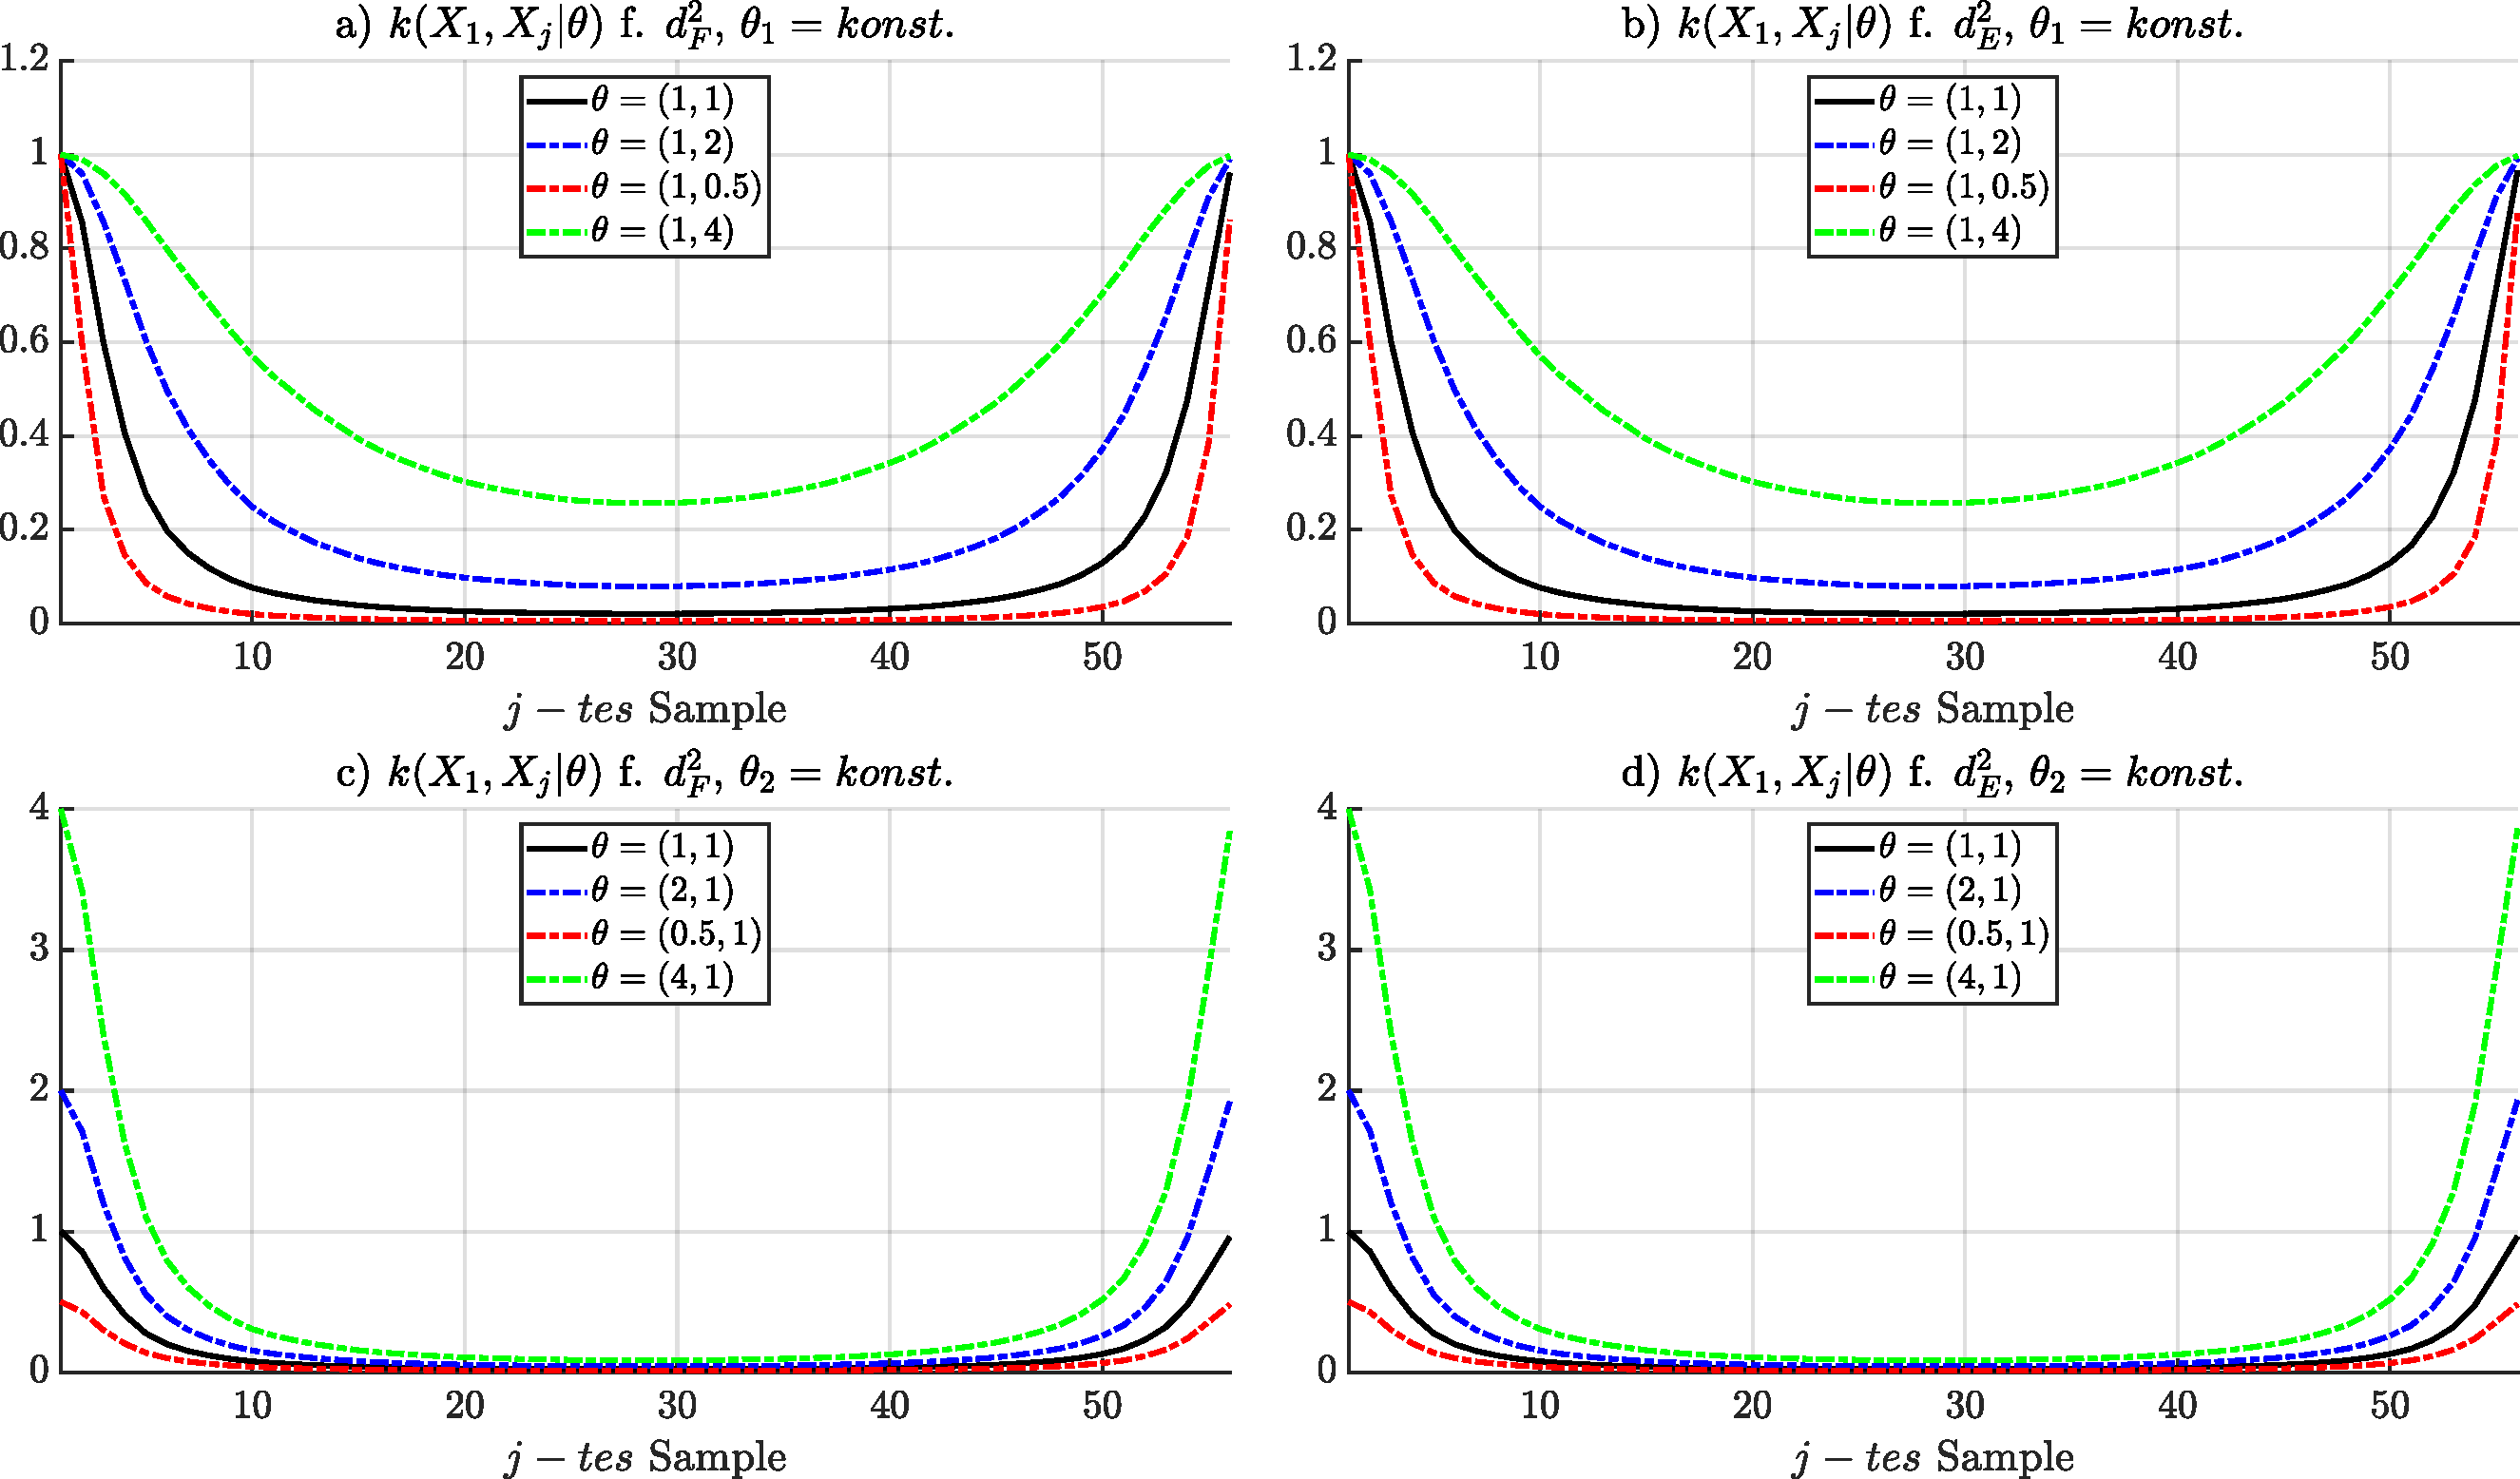
\includegraphics[width=\linewidth]{appendix/images/8-Ergebnisse-Experimente/Vergleich-Kovarianzfunktionen}
	\caption[Kovarianzfunktionen im Vergleich]{Kovarianzfunktionen im Vergleich für variierende Kernel-Parameter $\theta = (\sigma_f^2, \sigma_l)$ und $N=56$ Observerierungen.}
	\label{fig:vergleich-kovarianzfunktionen}
\end{figure}



\begin{figure}[tbph]
	\centering
	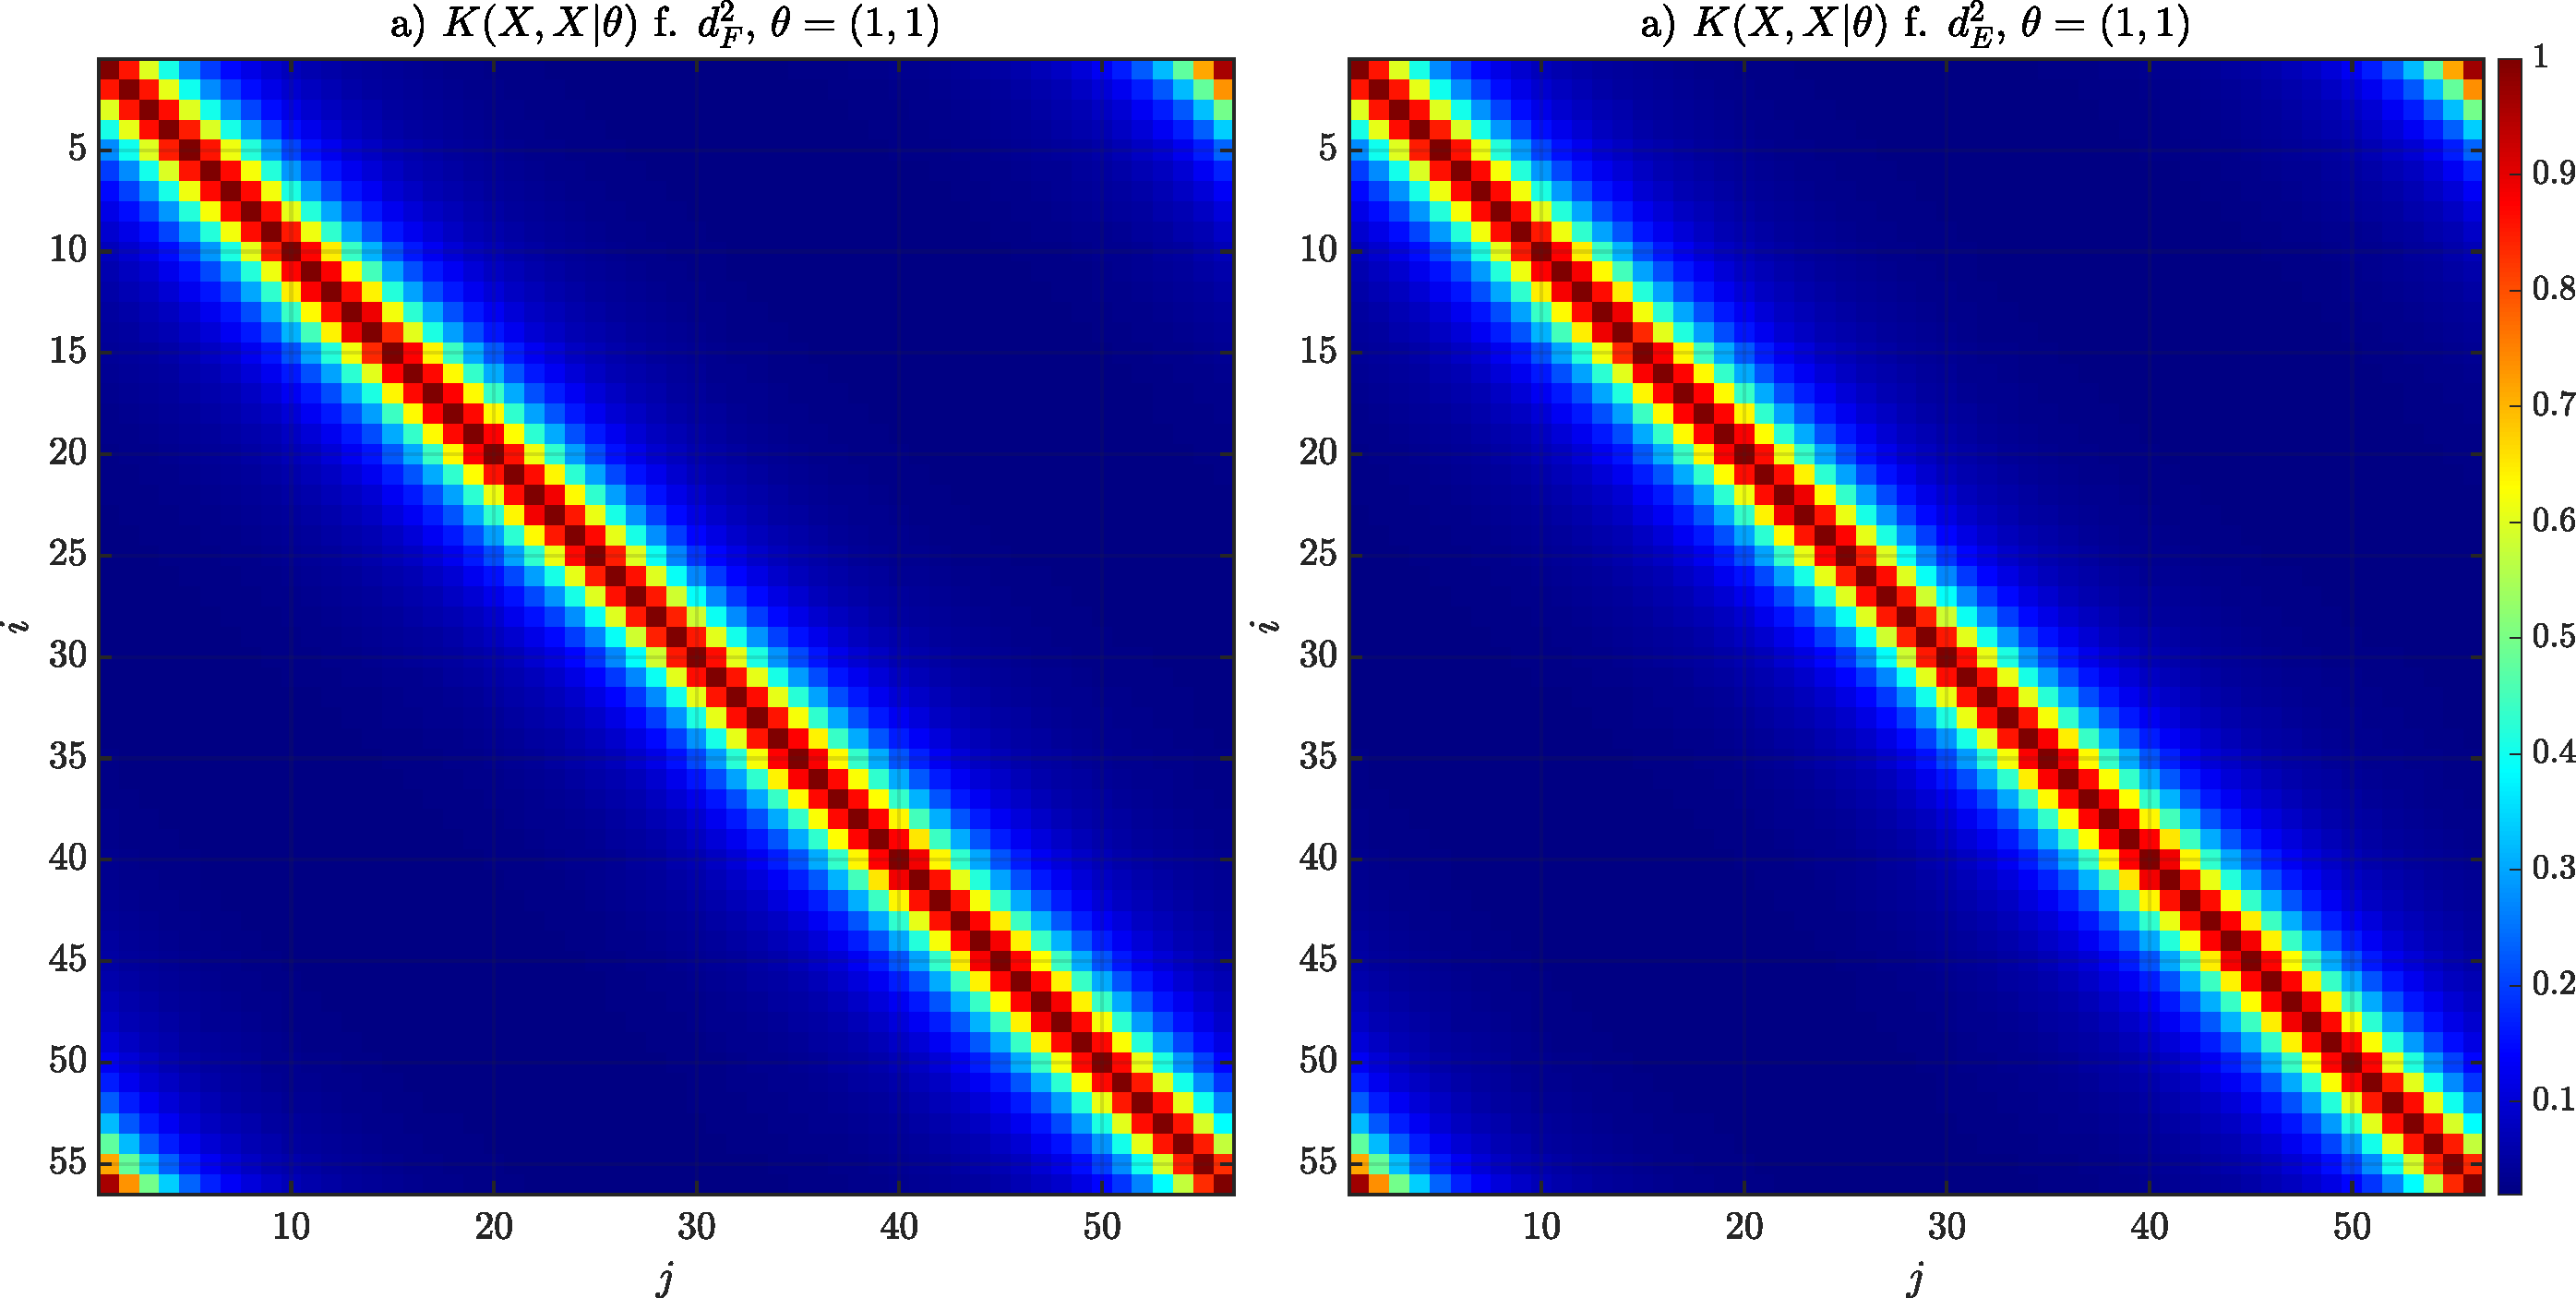
\includegraphics[width=\linewidth]{appendix/images/8-Ergebnisse-Experimente/Vergleich-Kovarianzmatrizen}
	\caption[Gegenüberstellung der Kovarianzmatrizen]{Gegenüberstellung der Kovarianzmatrizen bei ausgeschalter Längen- und und Breitenskalierung mit $\theta = (1,1)$ und $N=56$ Observerierungen.}
	\label{fig:vergleich-kovarianzmatrizen}
\end{figure}


\begin{figure}[tbph]
	\centering
	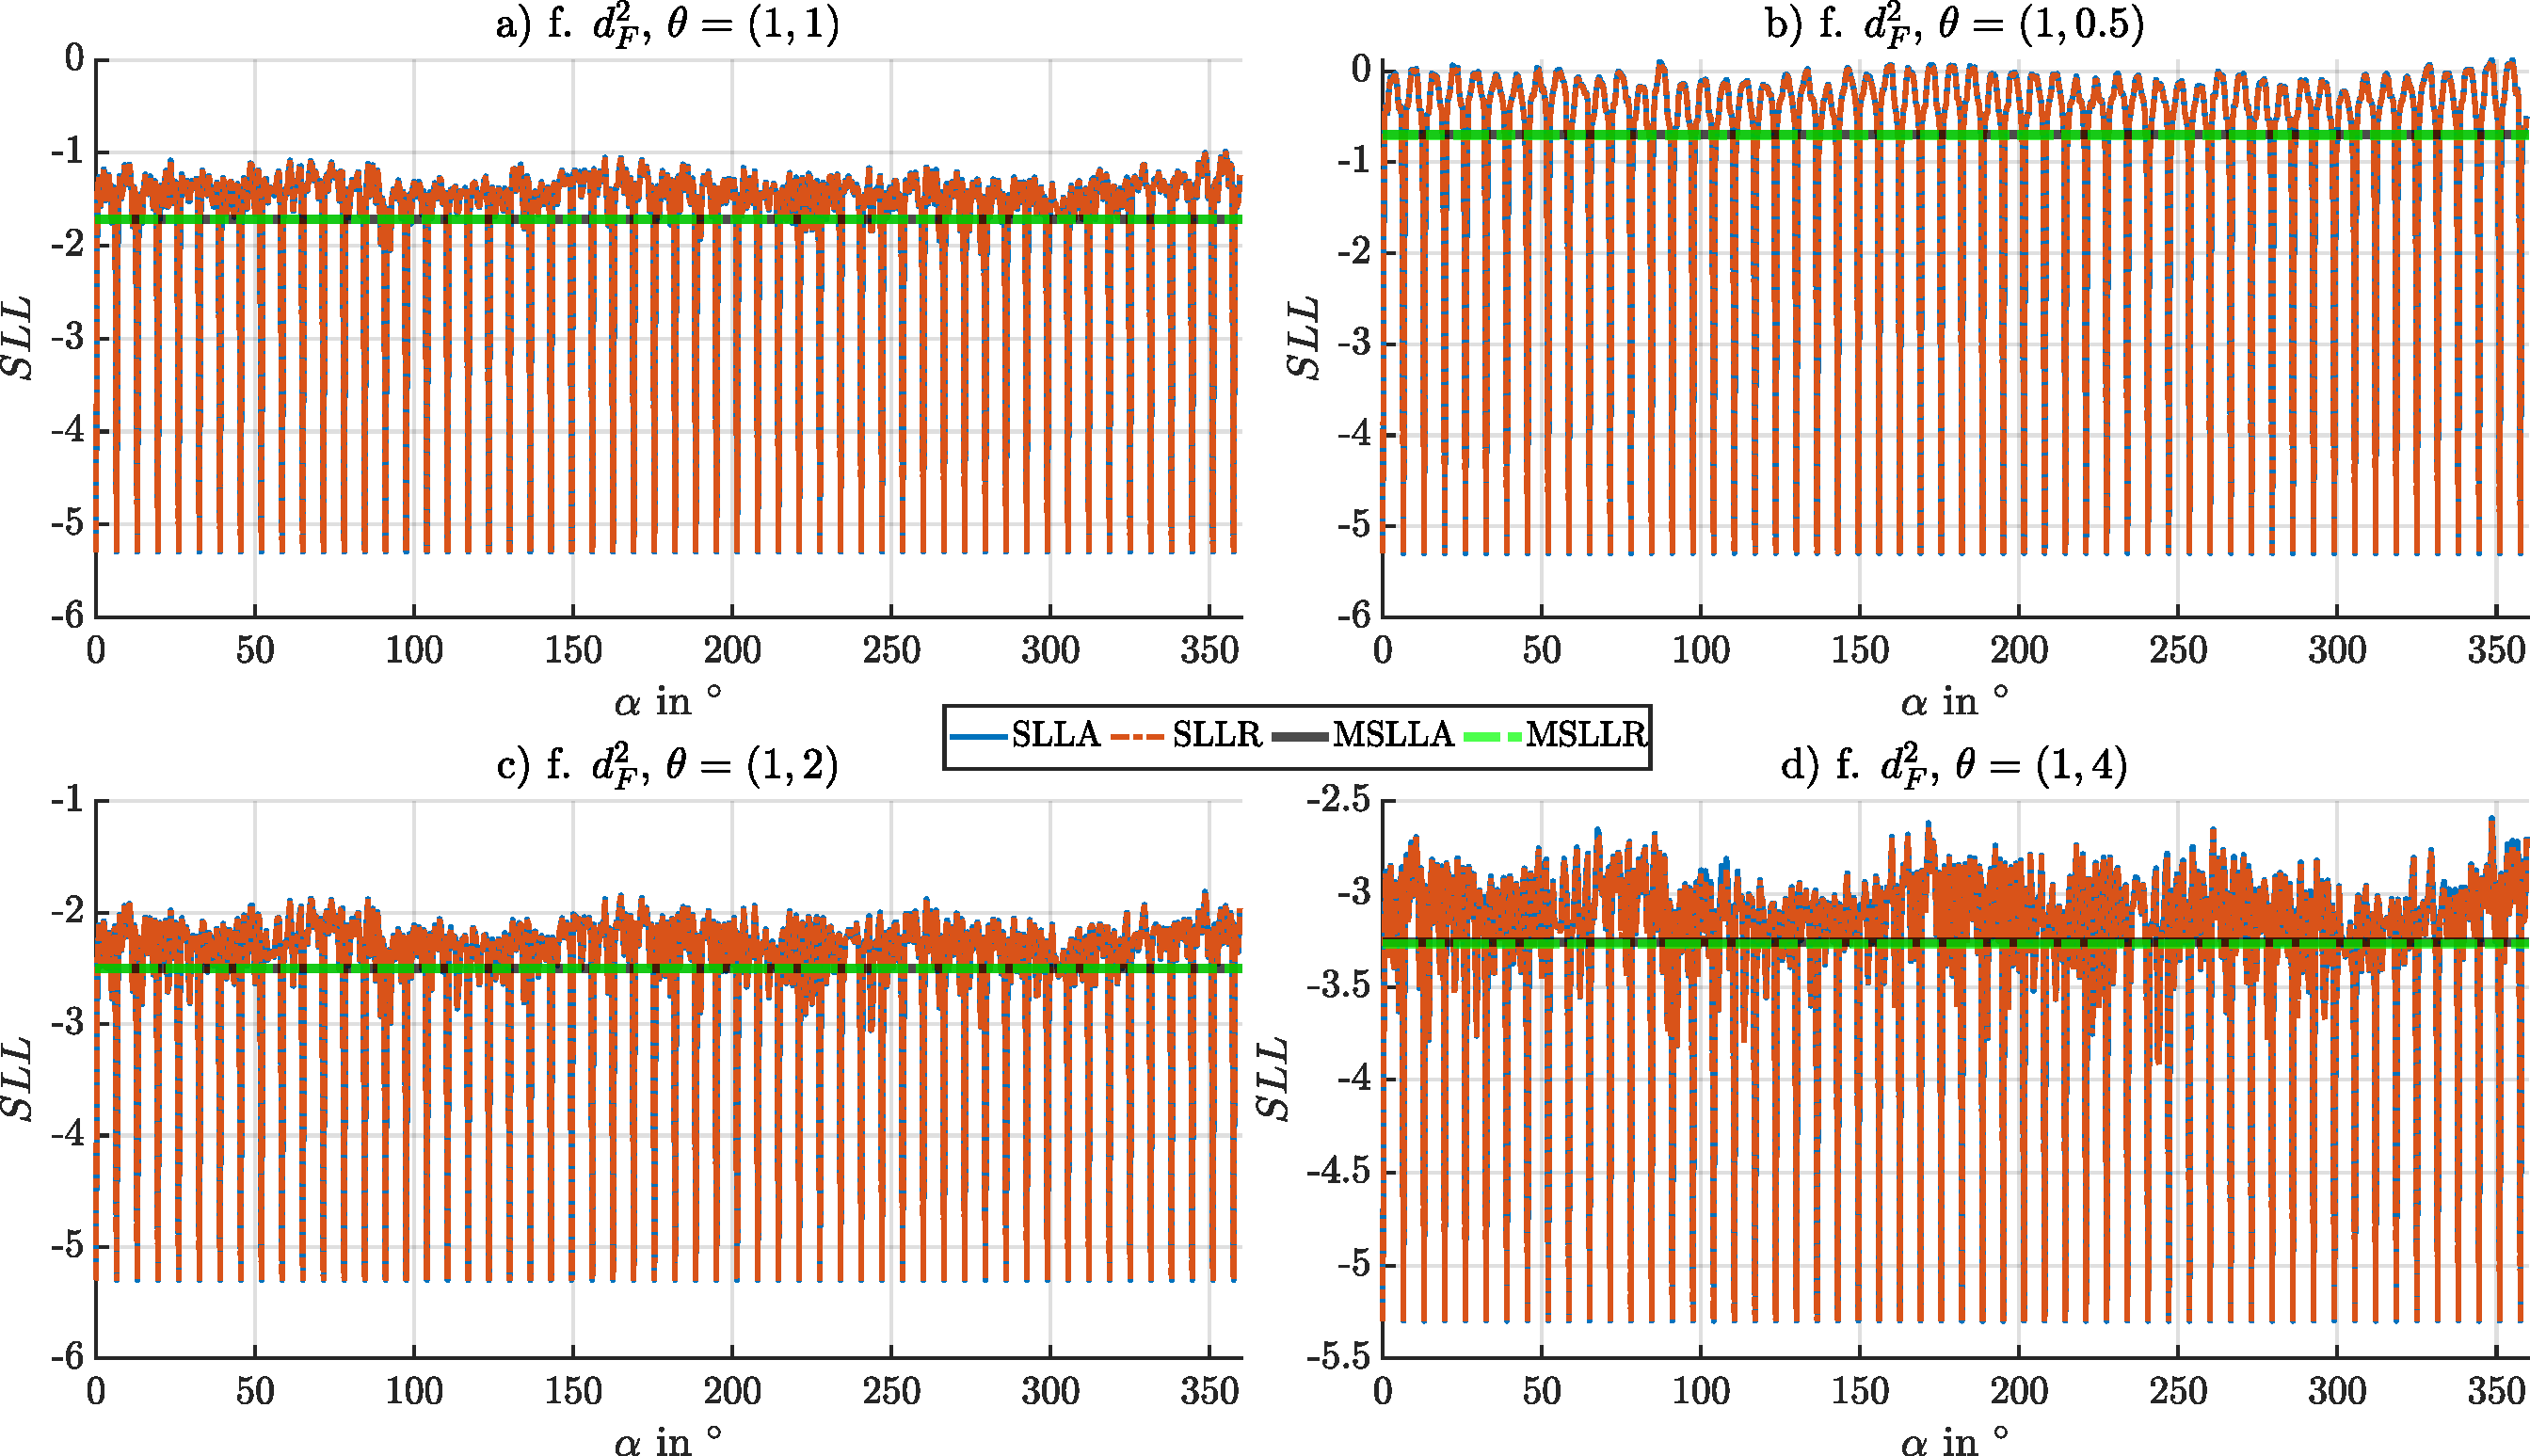
\includegraphics[width=\linewidth]{appendix/images/8-Ergebnisse-Experimente/Vergleich-QFC-SLL}
	\caption[Vergleich der Modellverluste nach Winkel und Radius für die erste Kovarianzfunktion]{Vergleich der Modellverluste nach Winkel und Radius für die erste Kovarianzfunktion für variierende Breitenskalierung.}
	\label{fig:vergleich-qfc-sll}
\end{figure}


\begin{figure}[tbph]
	\centering
	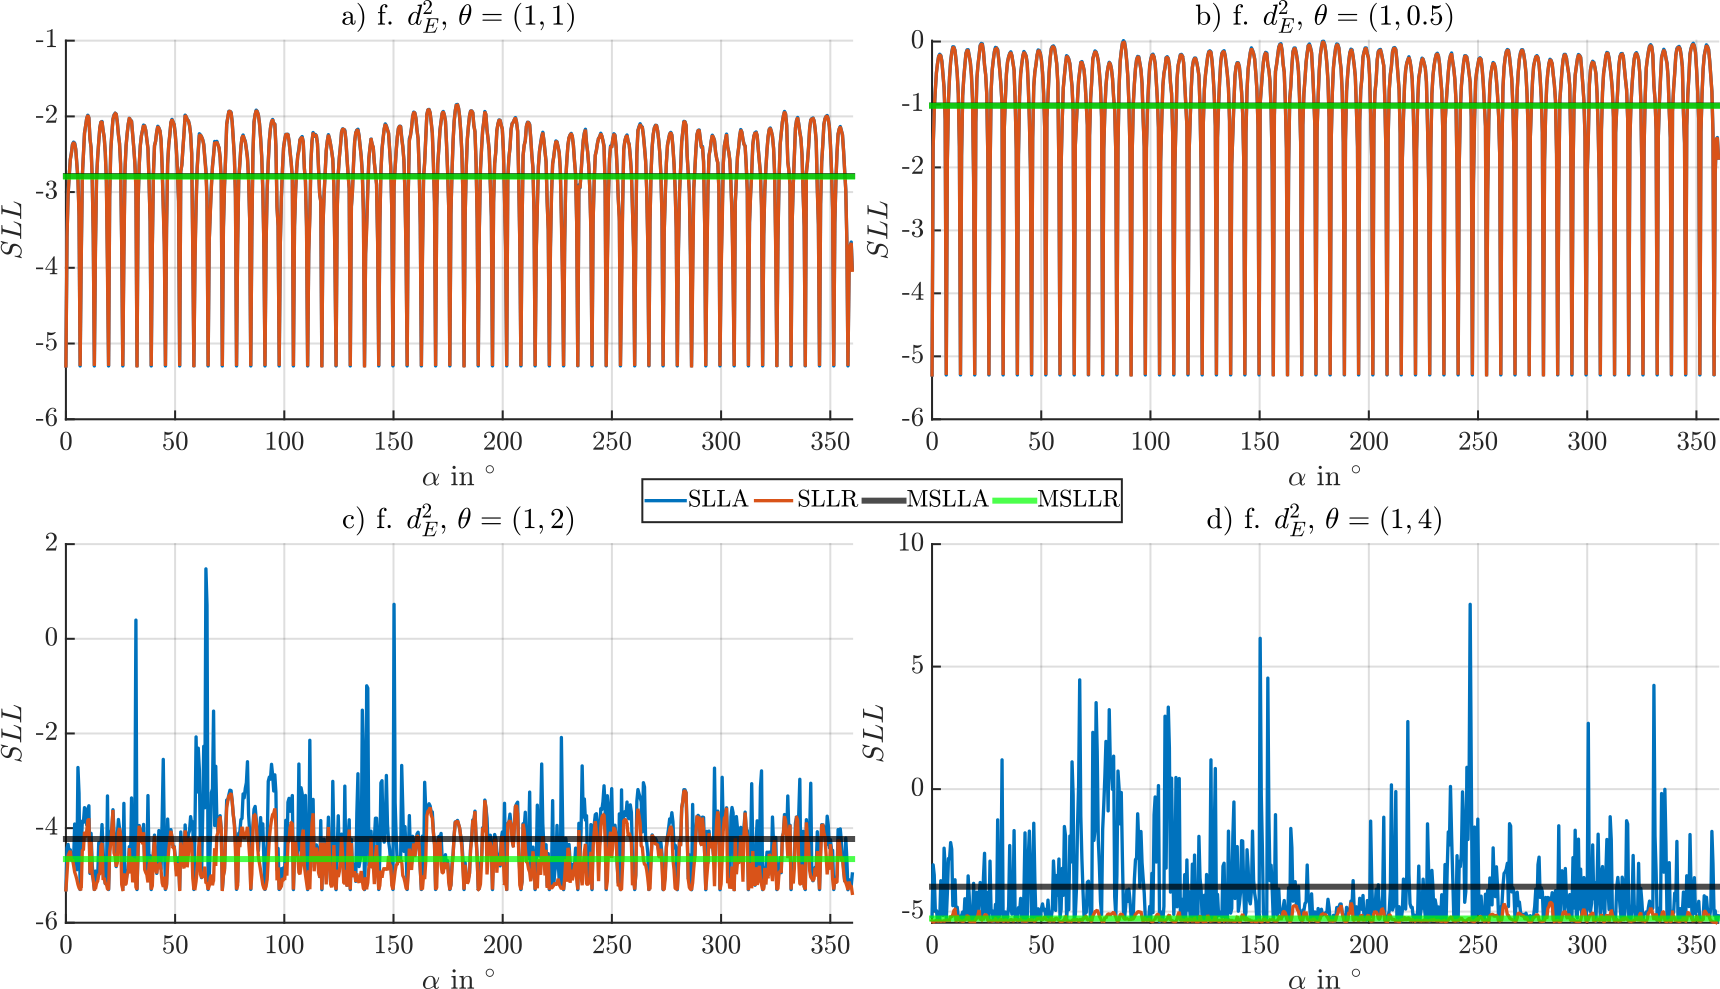
\includegraphics[width=\linewidth]{appendix/images/8-Ergebnisse-Experimente/Vergleich-QFCAPX-SLL}
	\caption[Vergleich der Modellverluste nach Winkel und Radius für die zweite Kovarianzfunktion]{Vergleich der Modellverluste nach Winkel und Radius für die zweite Kovarianzfunktion für variierende Breitenskalierung.}
	\label{fig:vergleich-qfcapx-sll}
\end{figure}


\clearpage


\section{Anpassung der Referenzwinkelanzahl}\label{sec:ergexp2}


\begin{figure}[tbph]
	\centering
	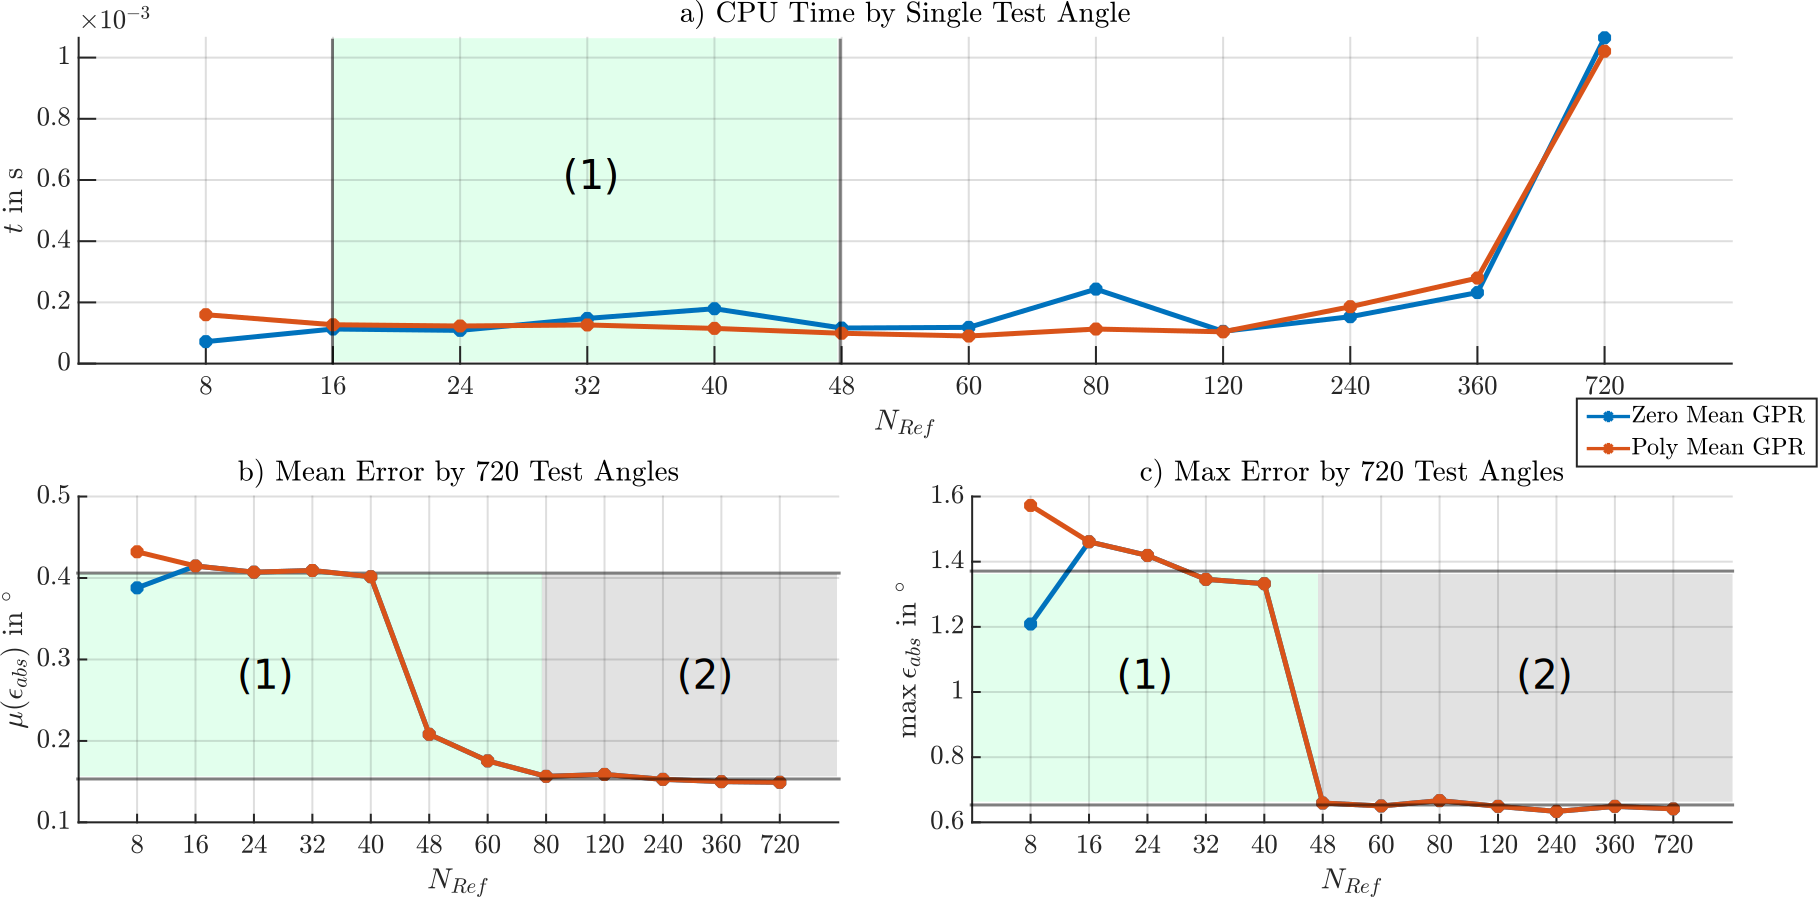
\includegraphics[width=\linewidth]{appendix/images/8-Ergebnisse-Experimente/Timings-vs-Errors}
	\caption[Timing vs Error]{QFCAPX Zero vs Poly 1 Nref Opt 32 (APX) = 8 (QFC) Timing vs Error, Noise Level Gap äußere Optimierung gleicht aus. (1) zu wählender Bereich mit 32 Samples, erfordert Rauschanpassung. (2) Rauschanpassung nicht zwingend notwendig, aber ressourcenintensiv.}
	\label{fig:timings-vs-errors}
\end{figure}


\clearpage


\section{Anpassung des Rauschniveaus}\label{sec:ergexp3}


\begin{figure}[tbph]
	\centering
	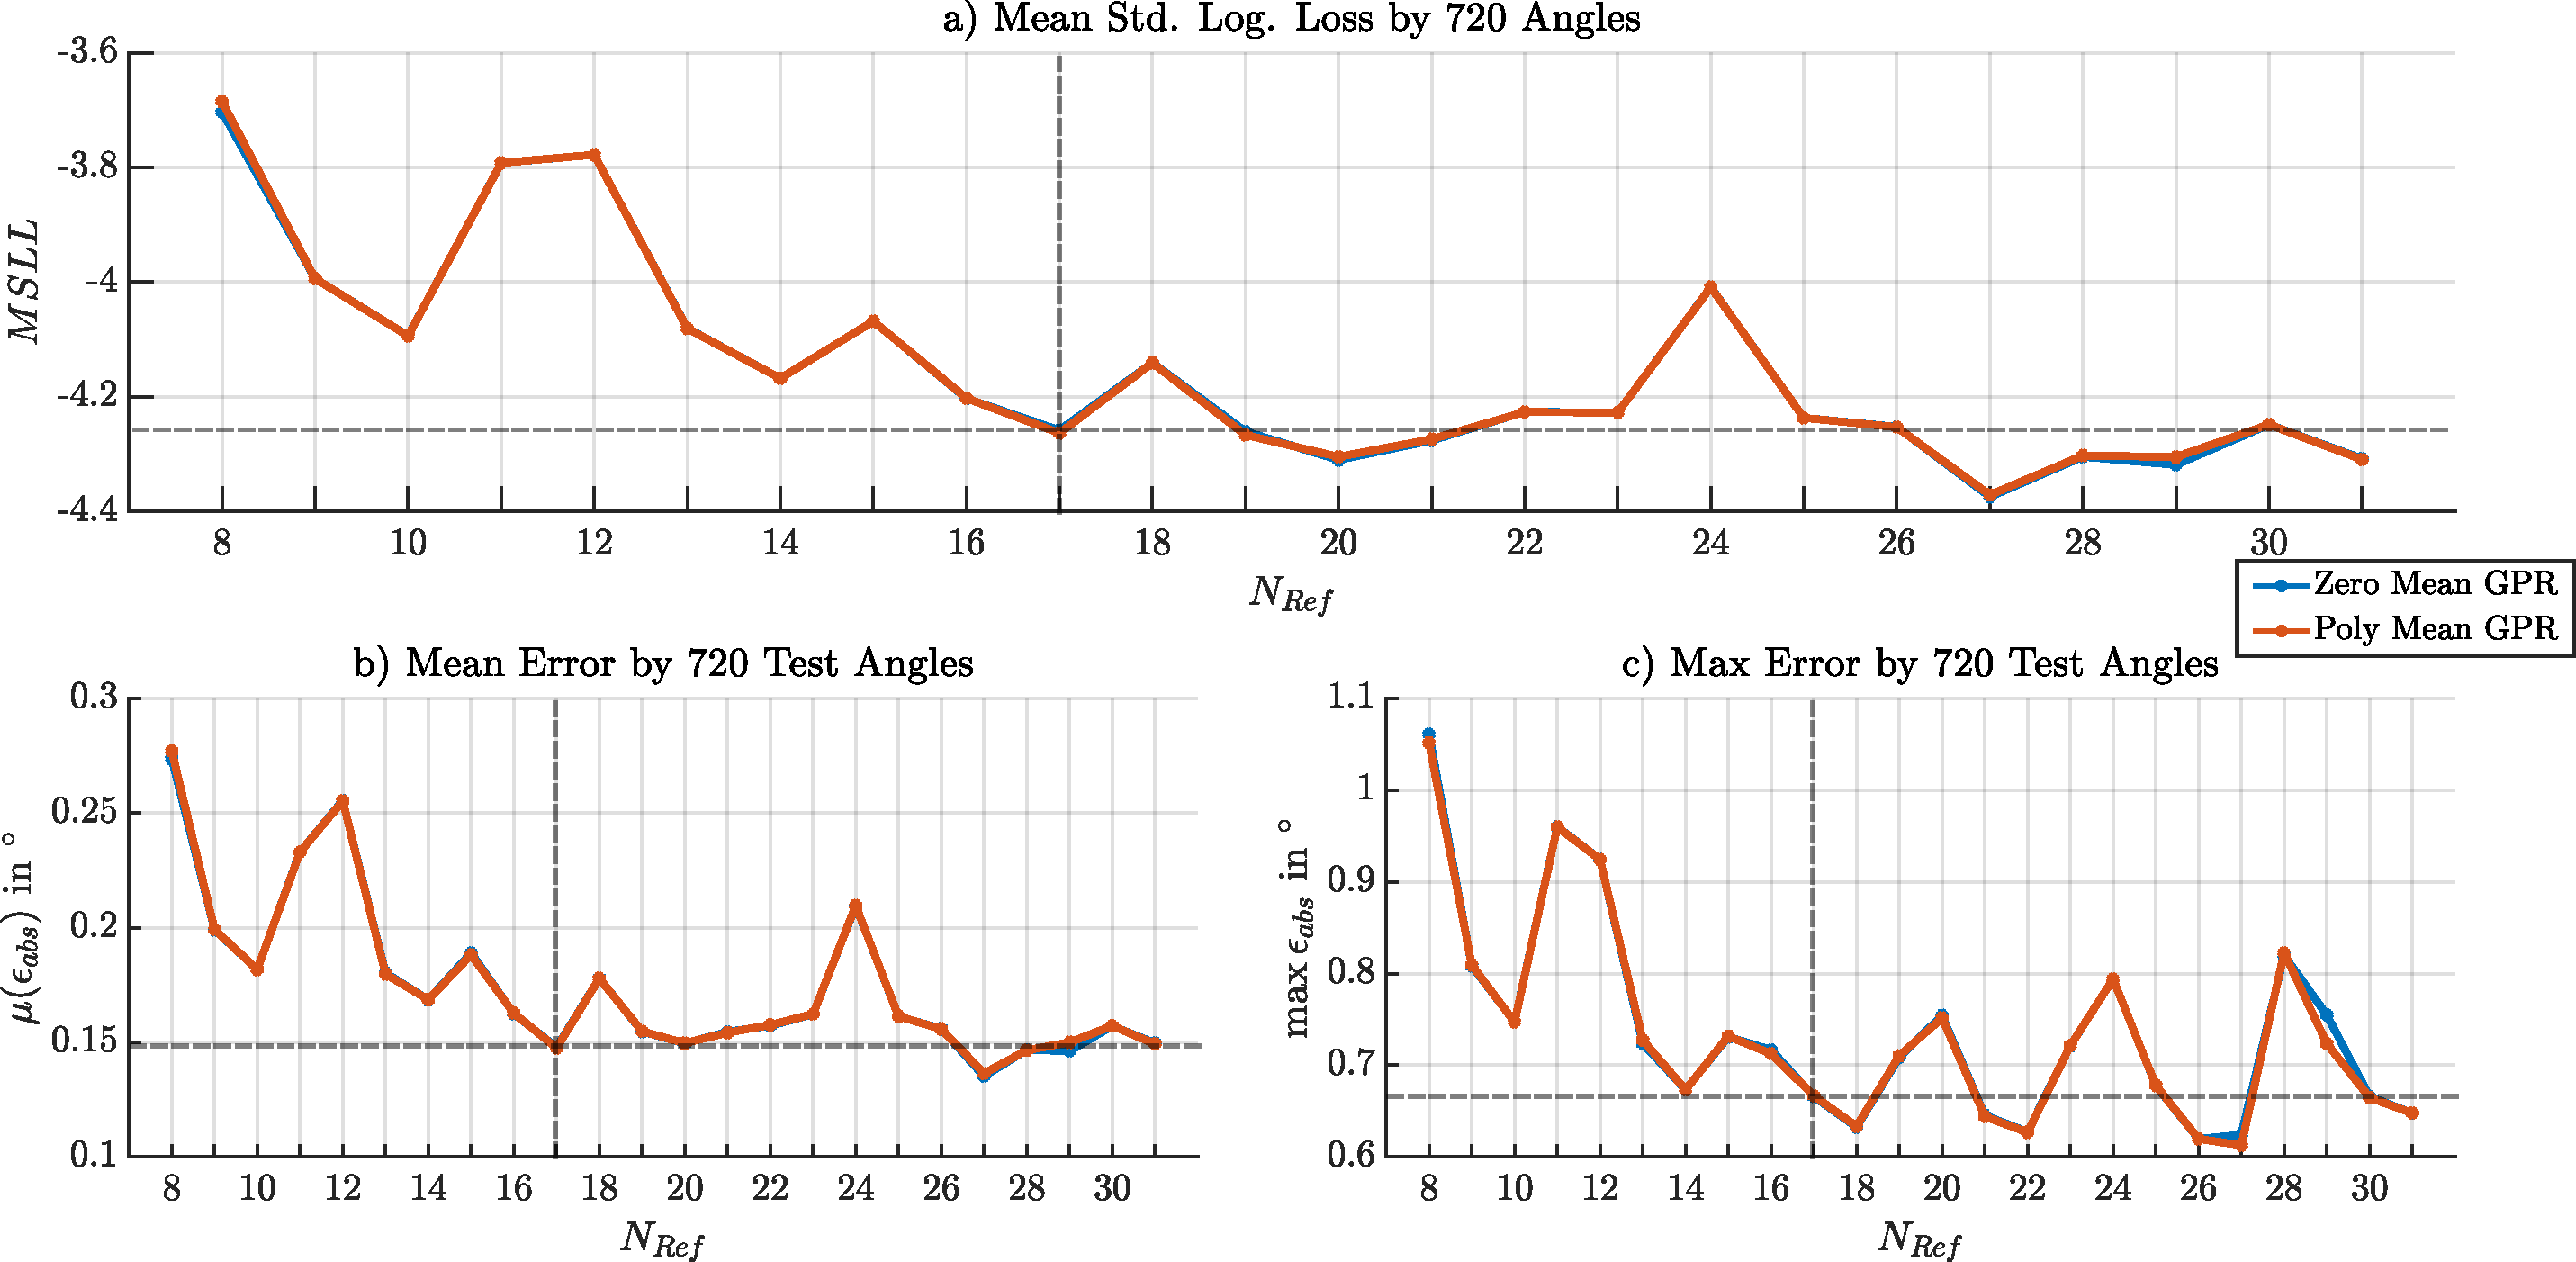
\includegraphics[width=\linewidth]{appendix/images/8-Ergebnisse-Experimente/MSLL-vs-Errors}
	\caption[MSLL vs Error für Nref 17]{MSLL vs Error für Nref 17 Kompromiss}
	\label{fig:msll-vs-errors}
\end{figure}


\clearpage


\section{Anpassung der Parametergrenzen}\label{sec:ergexp4}

Anpassung:

$\sigma_f^2$-Bounds: $(1, 10)$ / $\sigma_l$-Bounds: $(10, 30)$ / $\sigma_n^2$-Bounds: $(10^{-6}, 10^{-4})$


\begin{figure}[tbph]
	\centering
	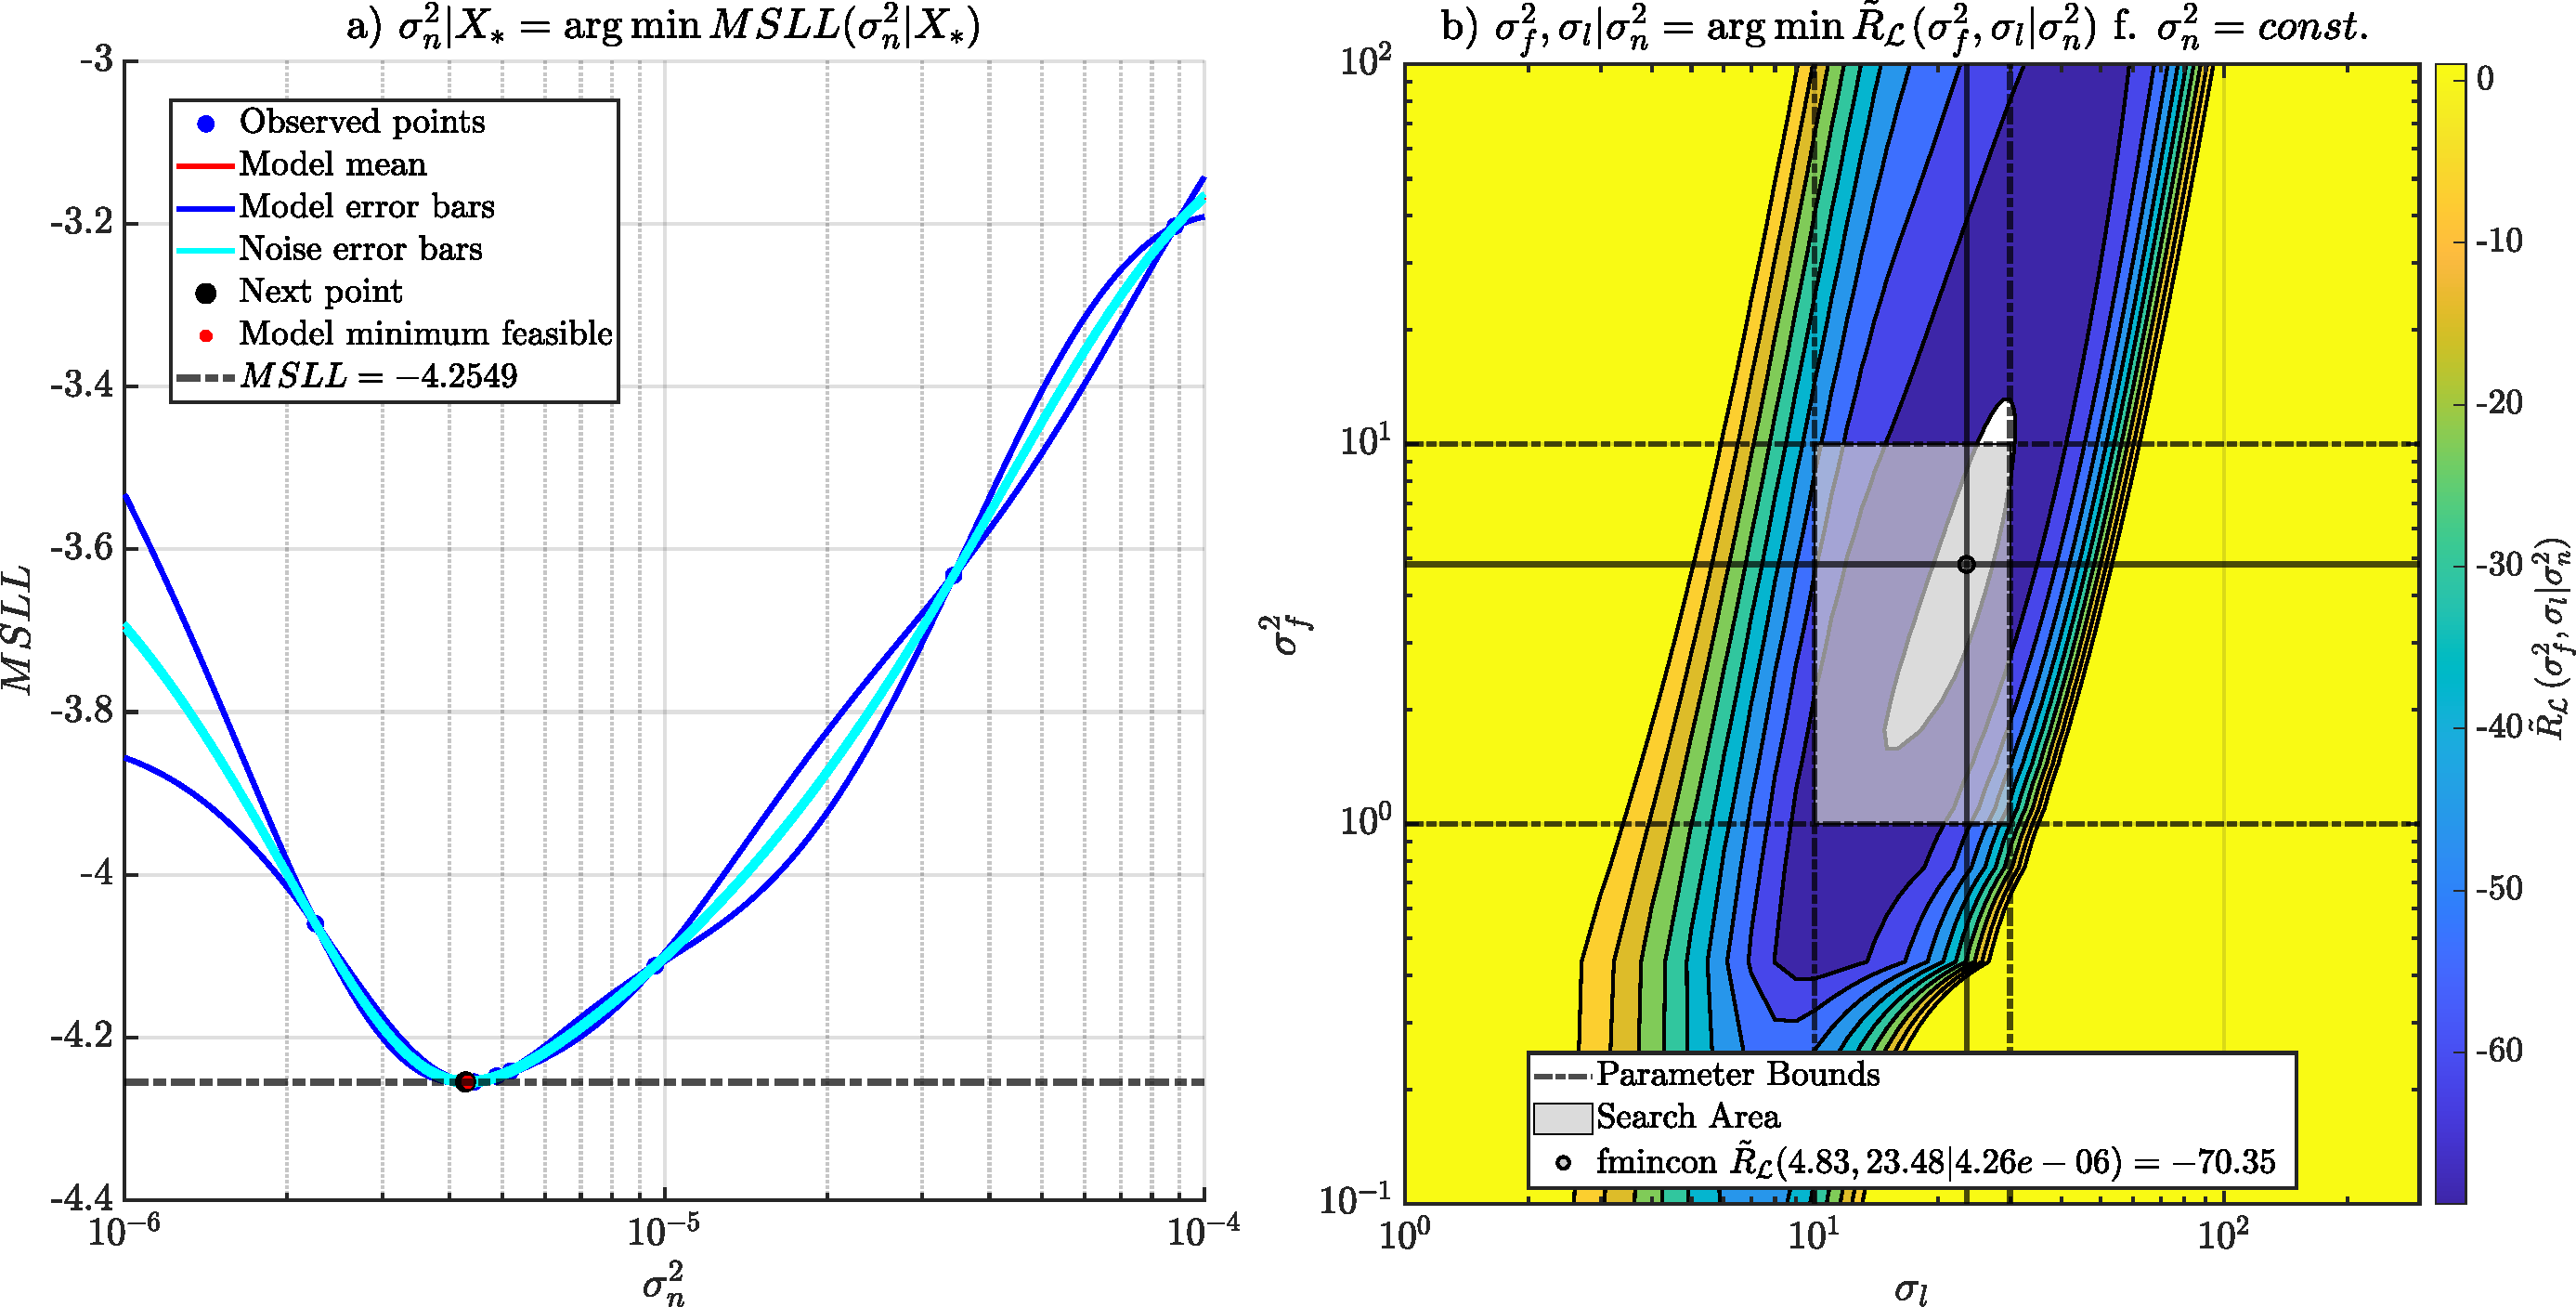
\includegraphics[width=\linewidth]{appendix/images/8-Ergebnisse-Experimente/QFCAPX-Z-N17-Bounds}
	\caption[Angepaster Parameter Bounds]{Angepaster Parameter Bounds}
	\label{fig:qfcapx-z-n17-bounds}
\end{figure}


Anpassung: Durchlaufzahl 10


\begin{figure}[tbph]
	\centering
	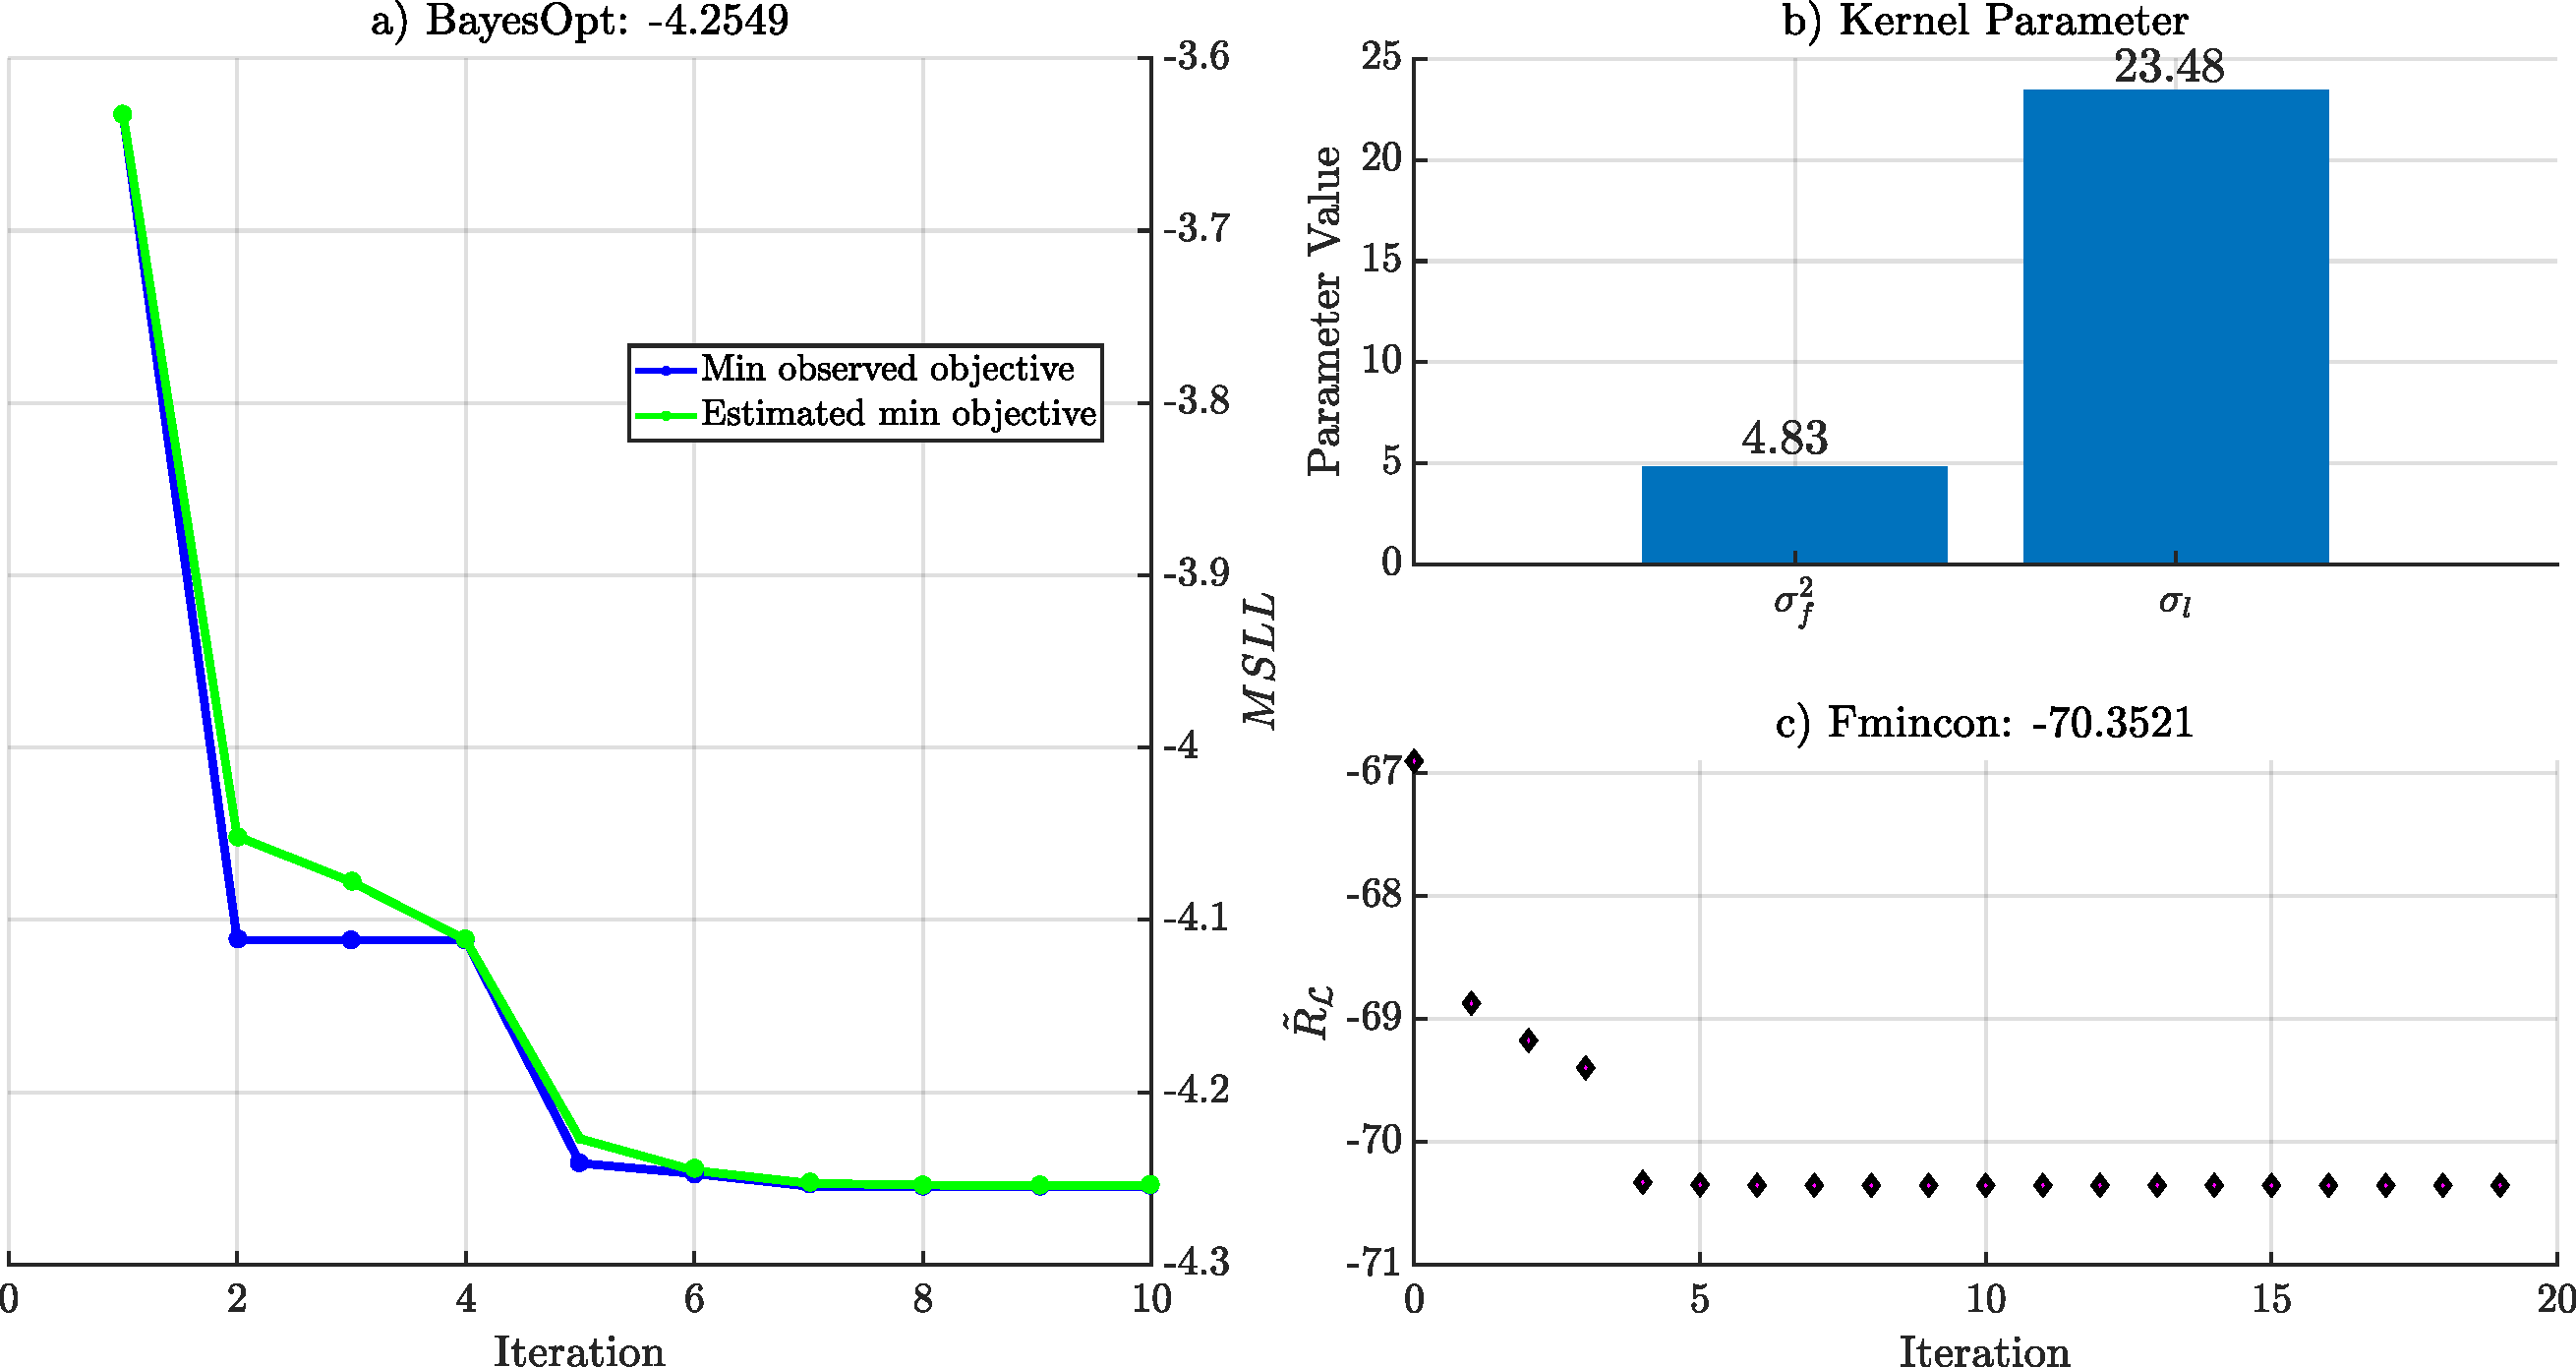
\includegraphics[width=\linewidth]{appendix/images/8-Ergebnisse-Experimente/QFCAPX-Z-N17-Opt}
	\caption[QFCAPX Z N17 Optimierung Runs 10]{QFCAPX Z N17 Optimierung Runs 10}
	\label{fig:qfcapx-z-n17-opt}
\end{figure}





\clearpage


\section{Verhalten bei einfachen Fehllagen}\label{sec:ergexp5}


\begin{figure}[tbph]
	\centering
	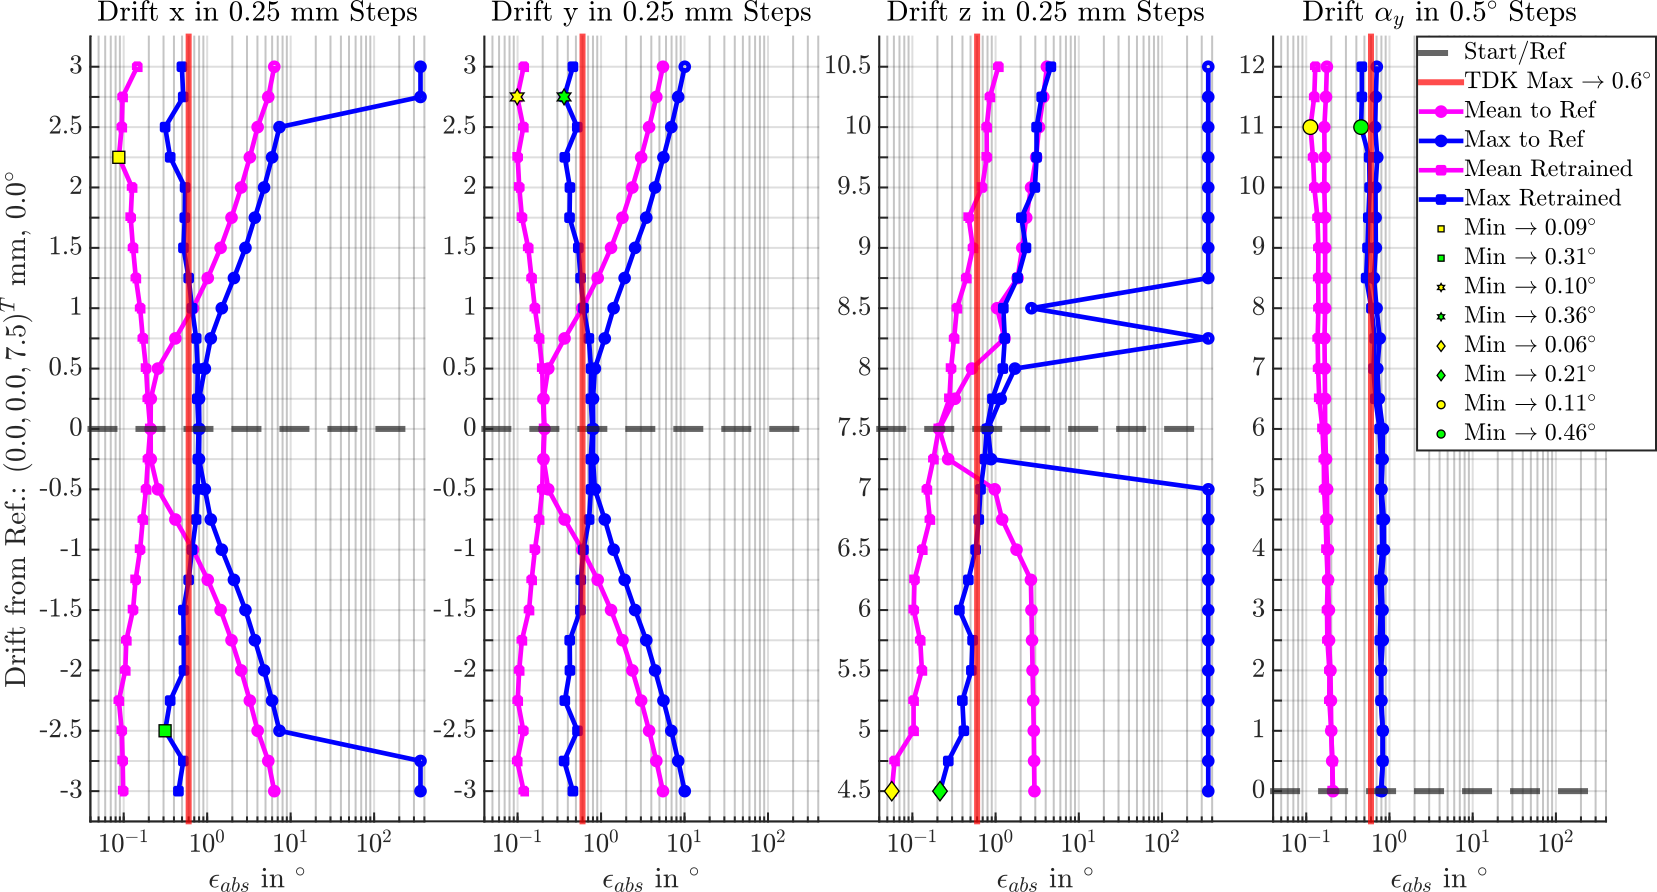
\includegraphics[width=\linewidth]{appendix/images/8-Ergebnisse-Experimente/Drift-Model-Errors}
	\caption[Drift xyz tilt mean max errors 2 ref and retrained]{Drift xyz tilt mean max errors 2 ref and retrained}
	\label{fig:drift-model-errors}
\end{figure}


\begin{figure}[tbph]
	\centering
	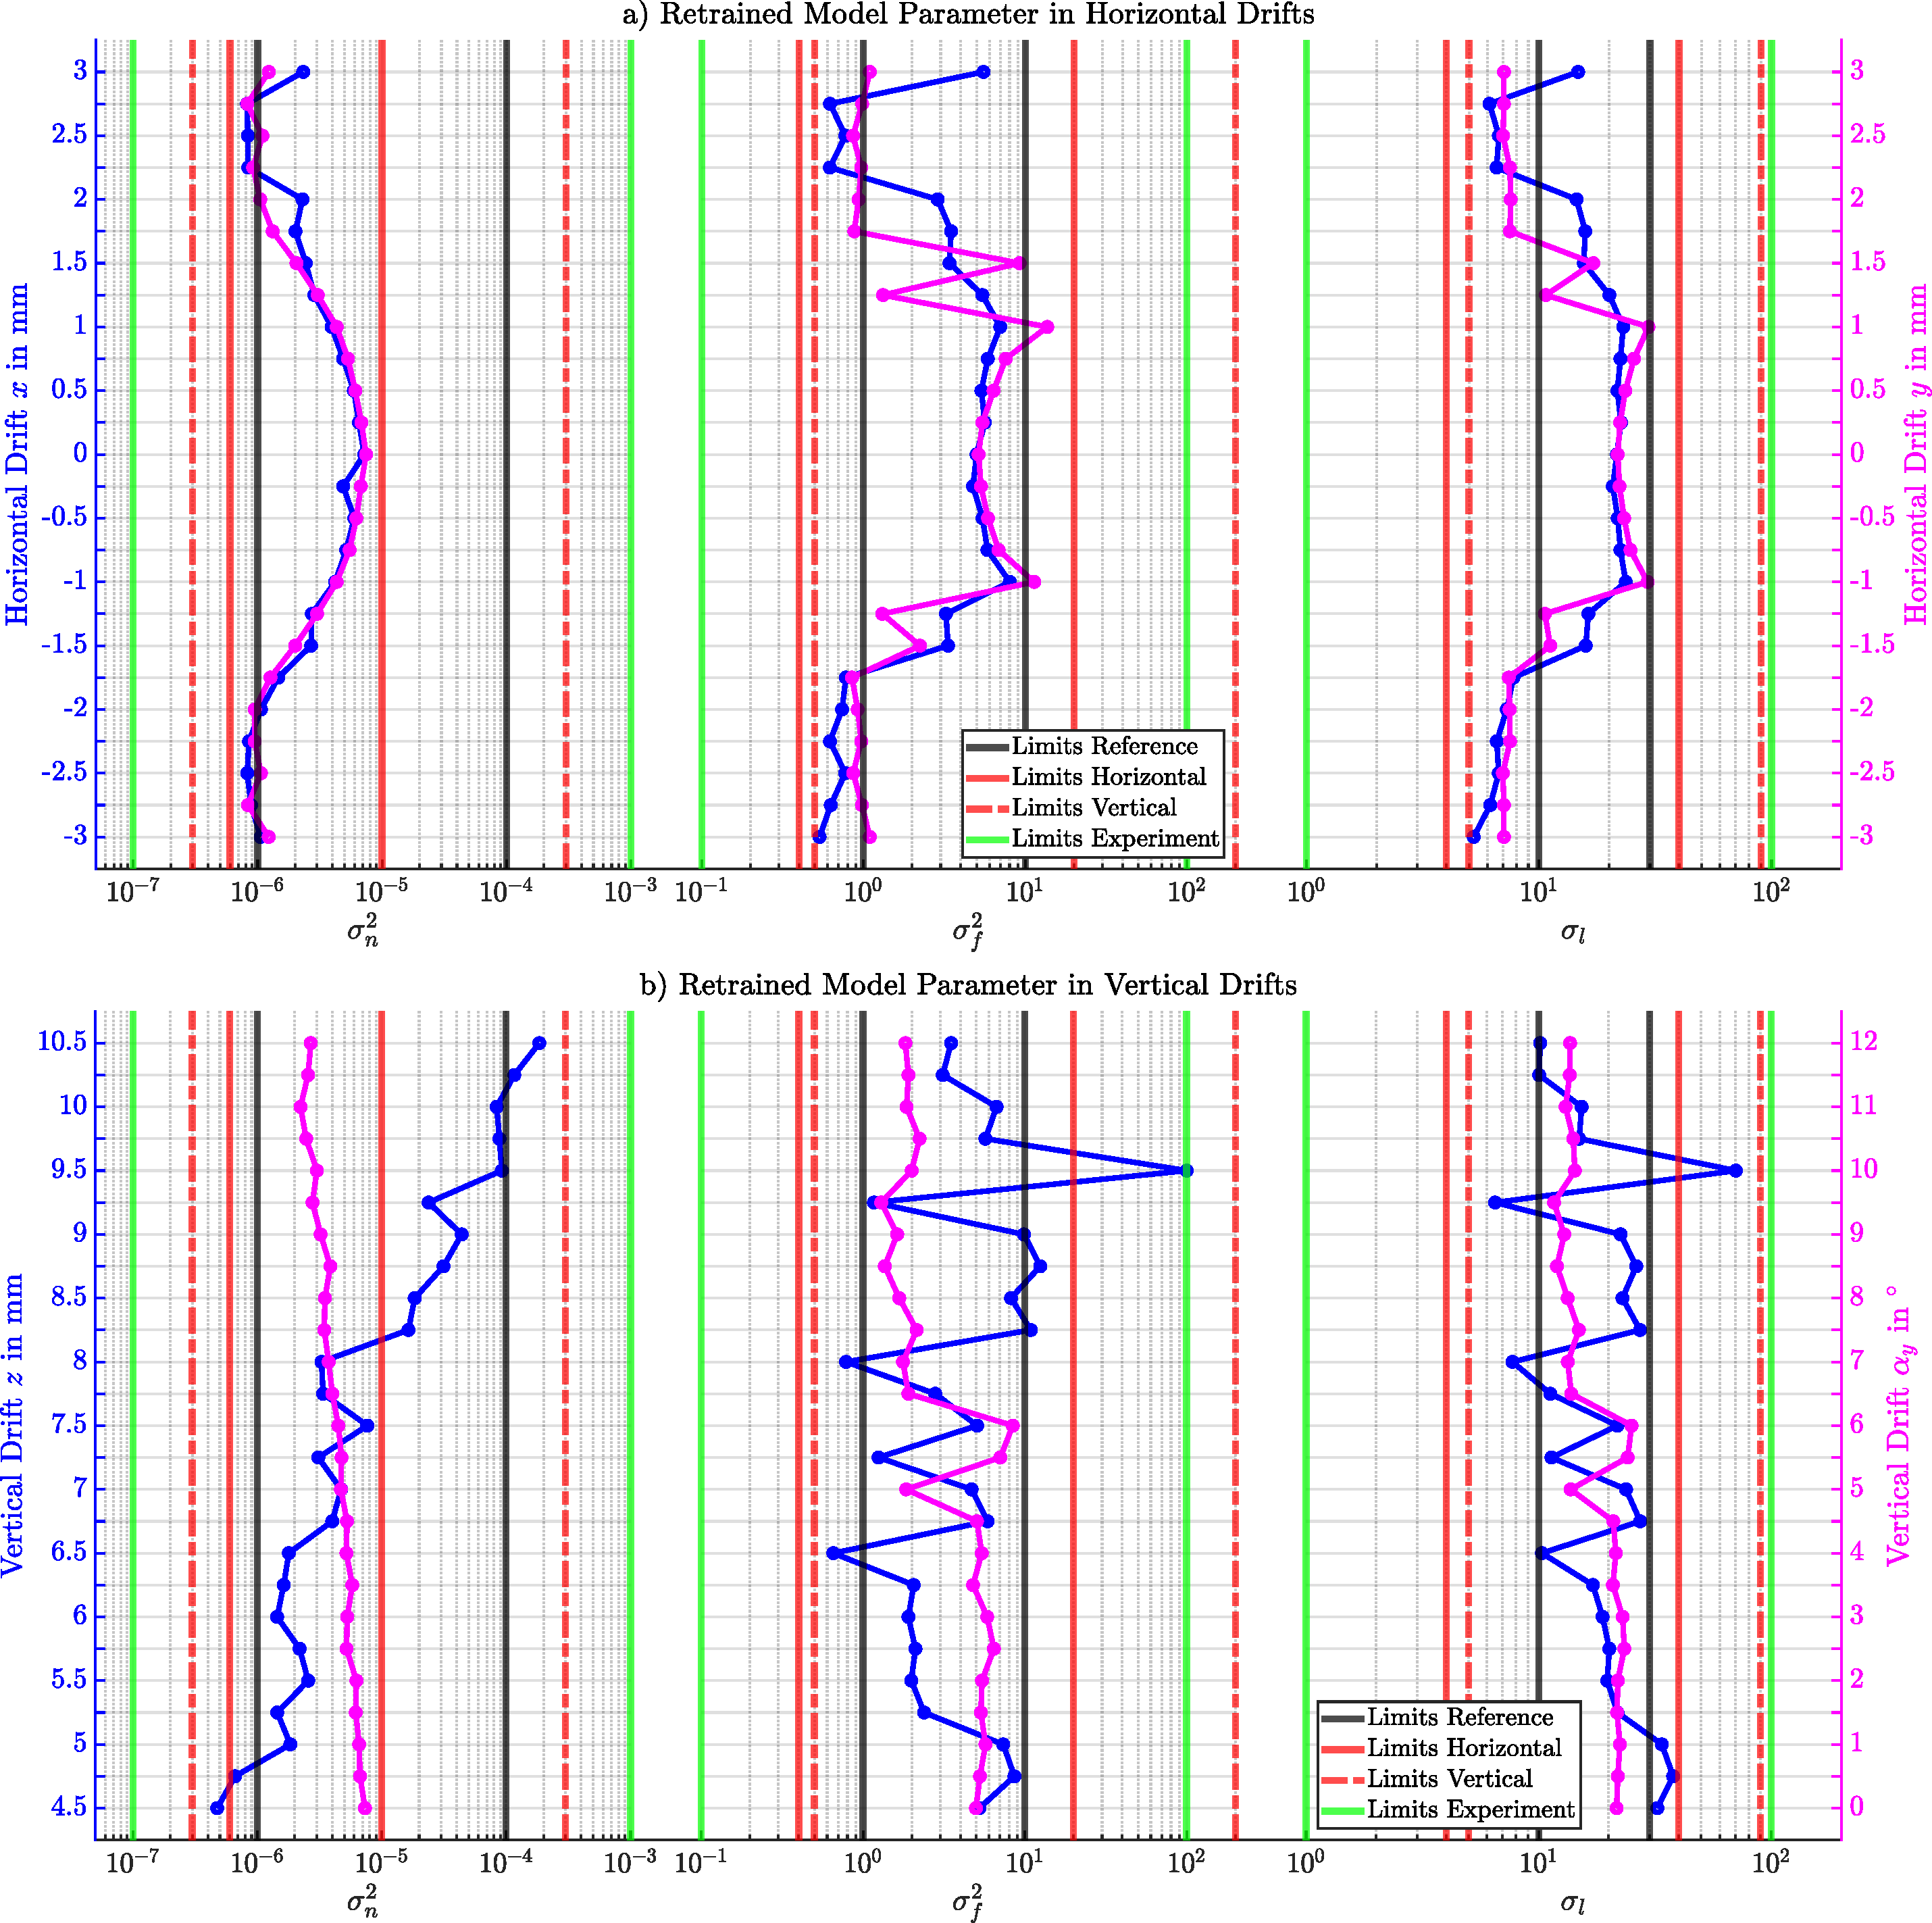
\includegraphics[width=\linewidth]{appendix/images/8-Ergebnisse-Experimente/Drift-Model-Parms}
	\caption[Drift xyz tilt retrained model params tracking]{Drift xyz tilt retrained model params tracking, limits from exp and ref and new suggestion}
	\label{fig:drift-model-parms}
\end{figure}


\begin{figure}[tbph]
	\centering
	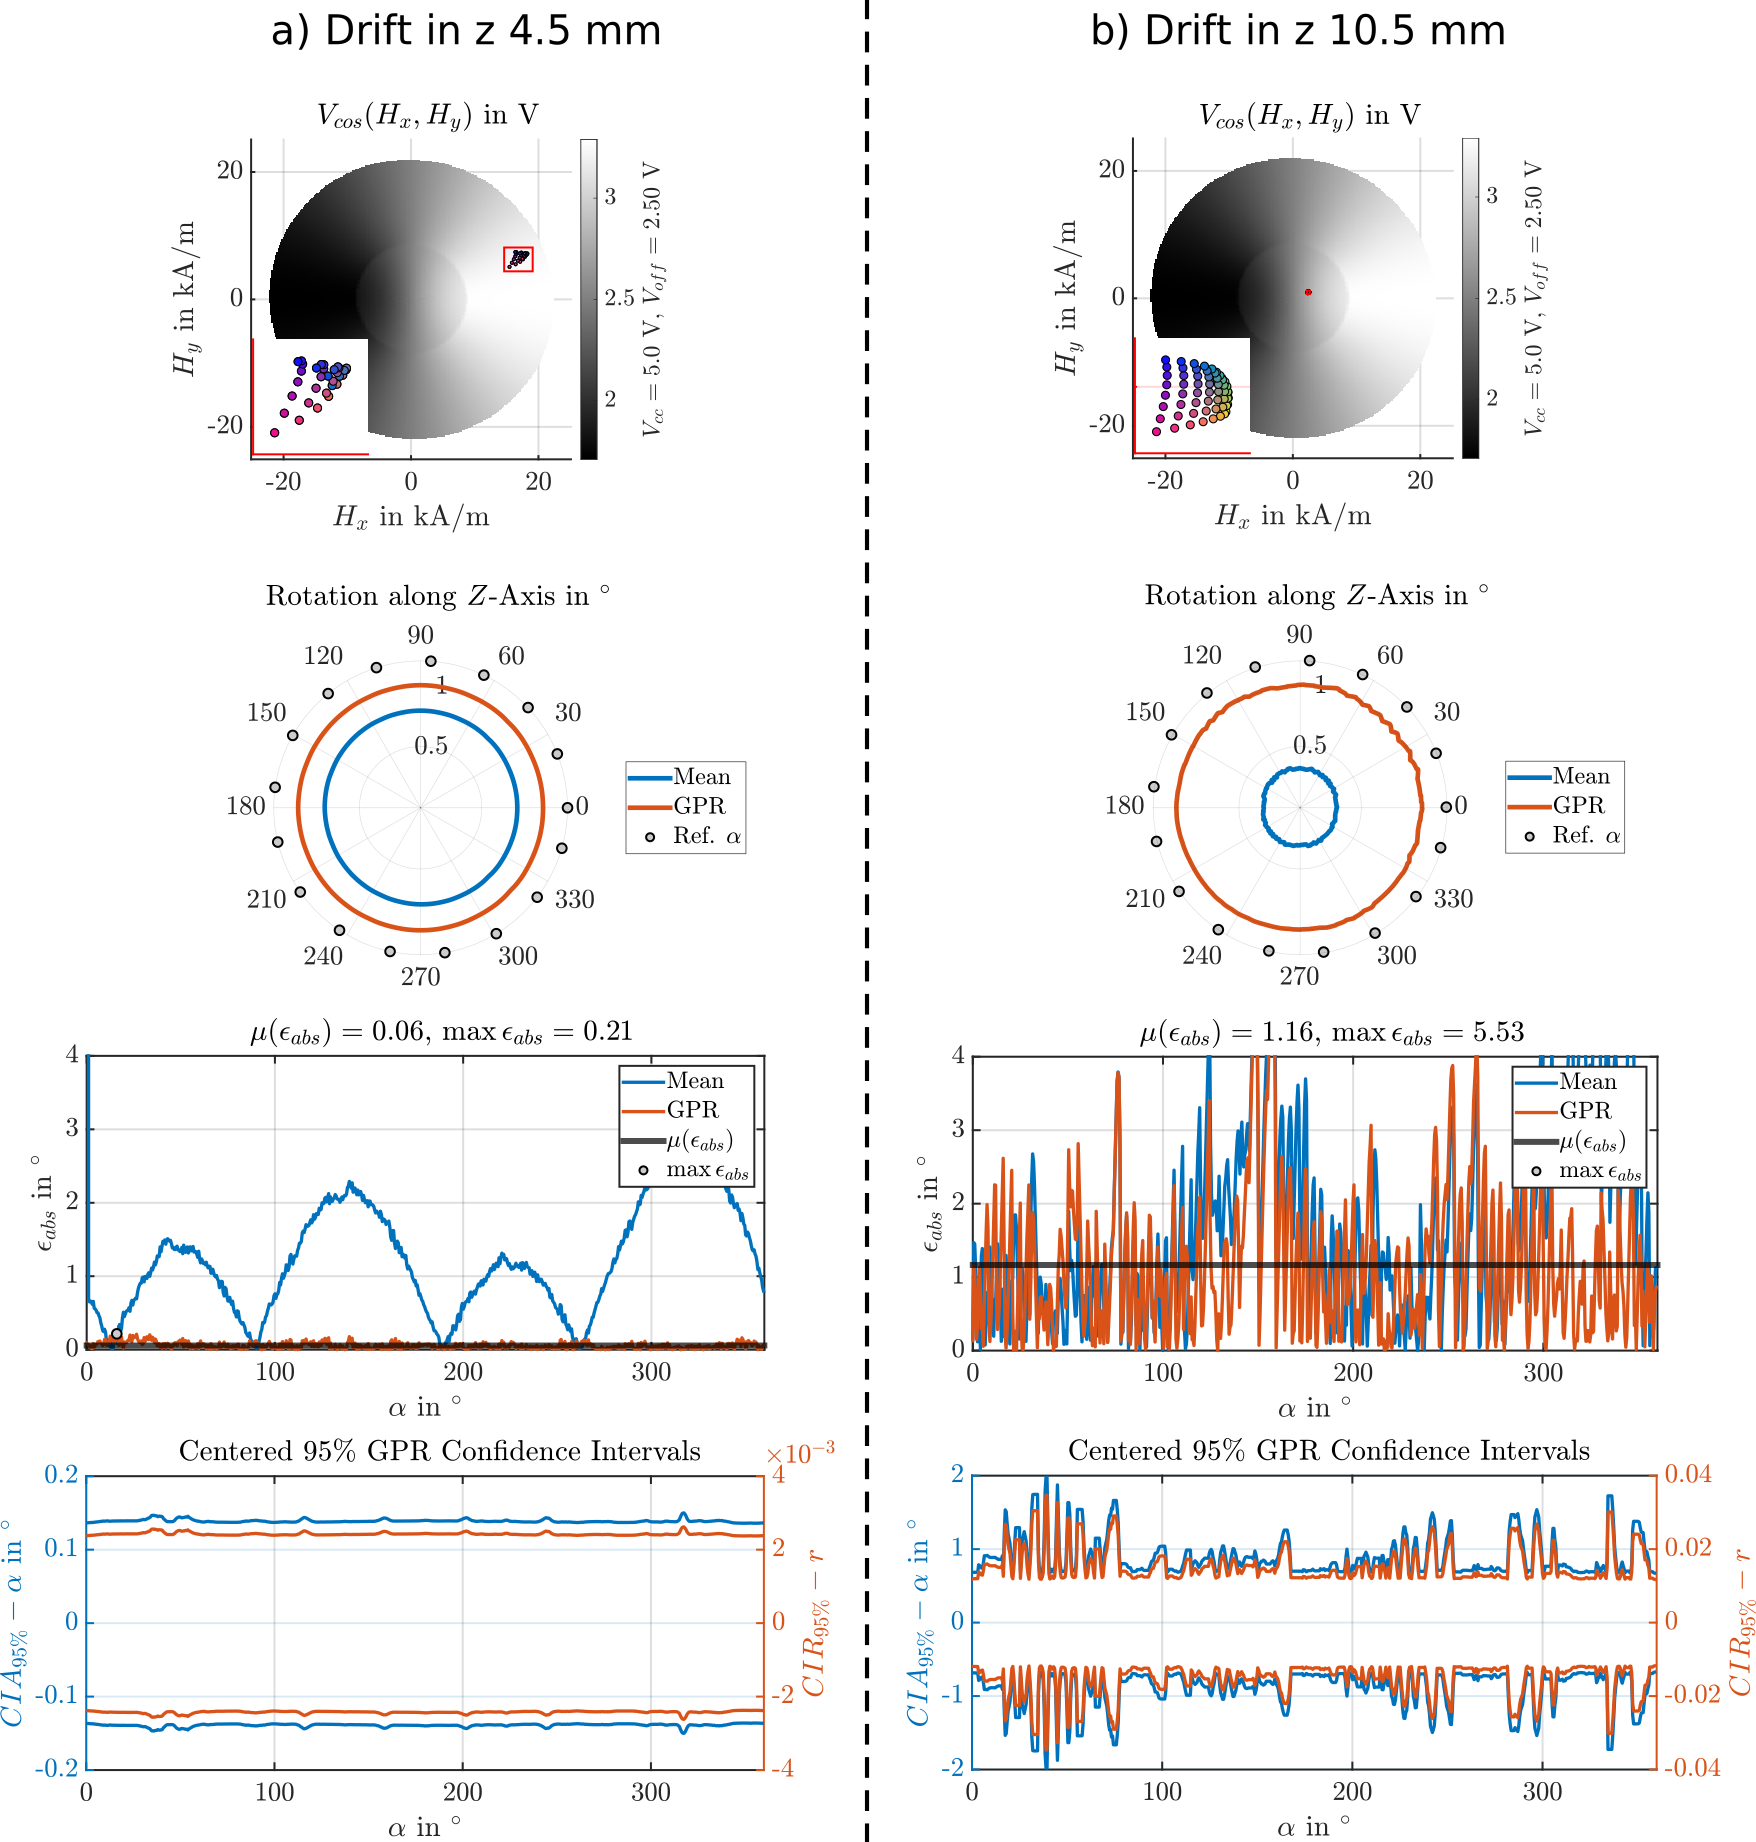
\includegraphics[width=\linewidth]{appendix/images/8-Ergebnisse-Experimente/Z-Pos-Comp-45-105-Rotation}
	\caption[Zpos 45 105 comp rotation]{Zpos a) 45 b) 105 comp rotation $\SI{21,5}{\degree}$ comp char spredding}
	\label{fig:z-pos-comp-45-105-rotation}
\end{figure}



\clearpage


\section{Verhalten bei kombinierten Fehllagen}\label{sec:ergexp6}

\begin{figure}[tbph]
	\centering
	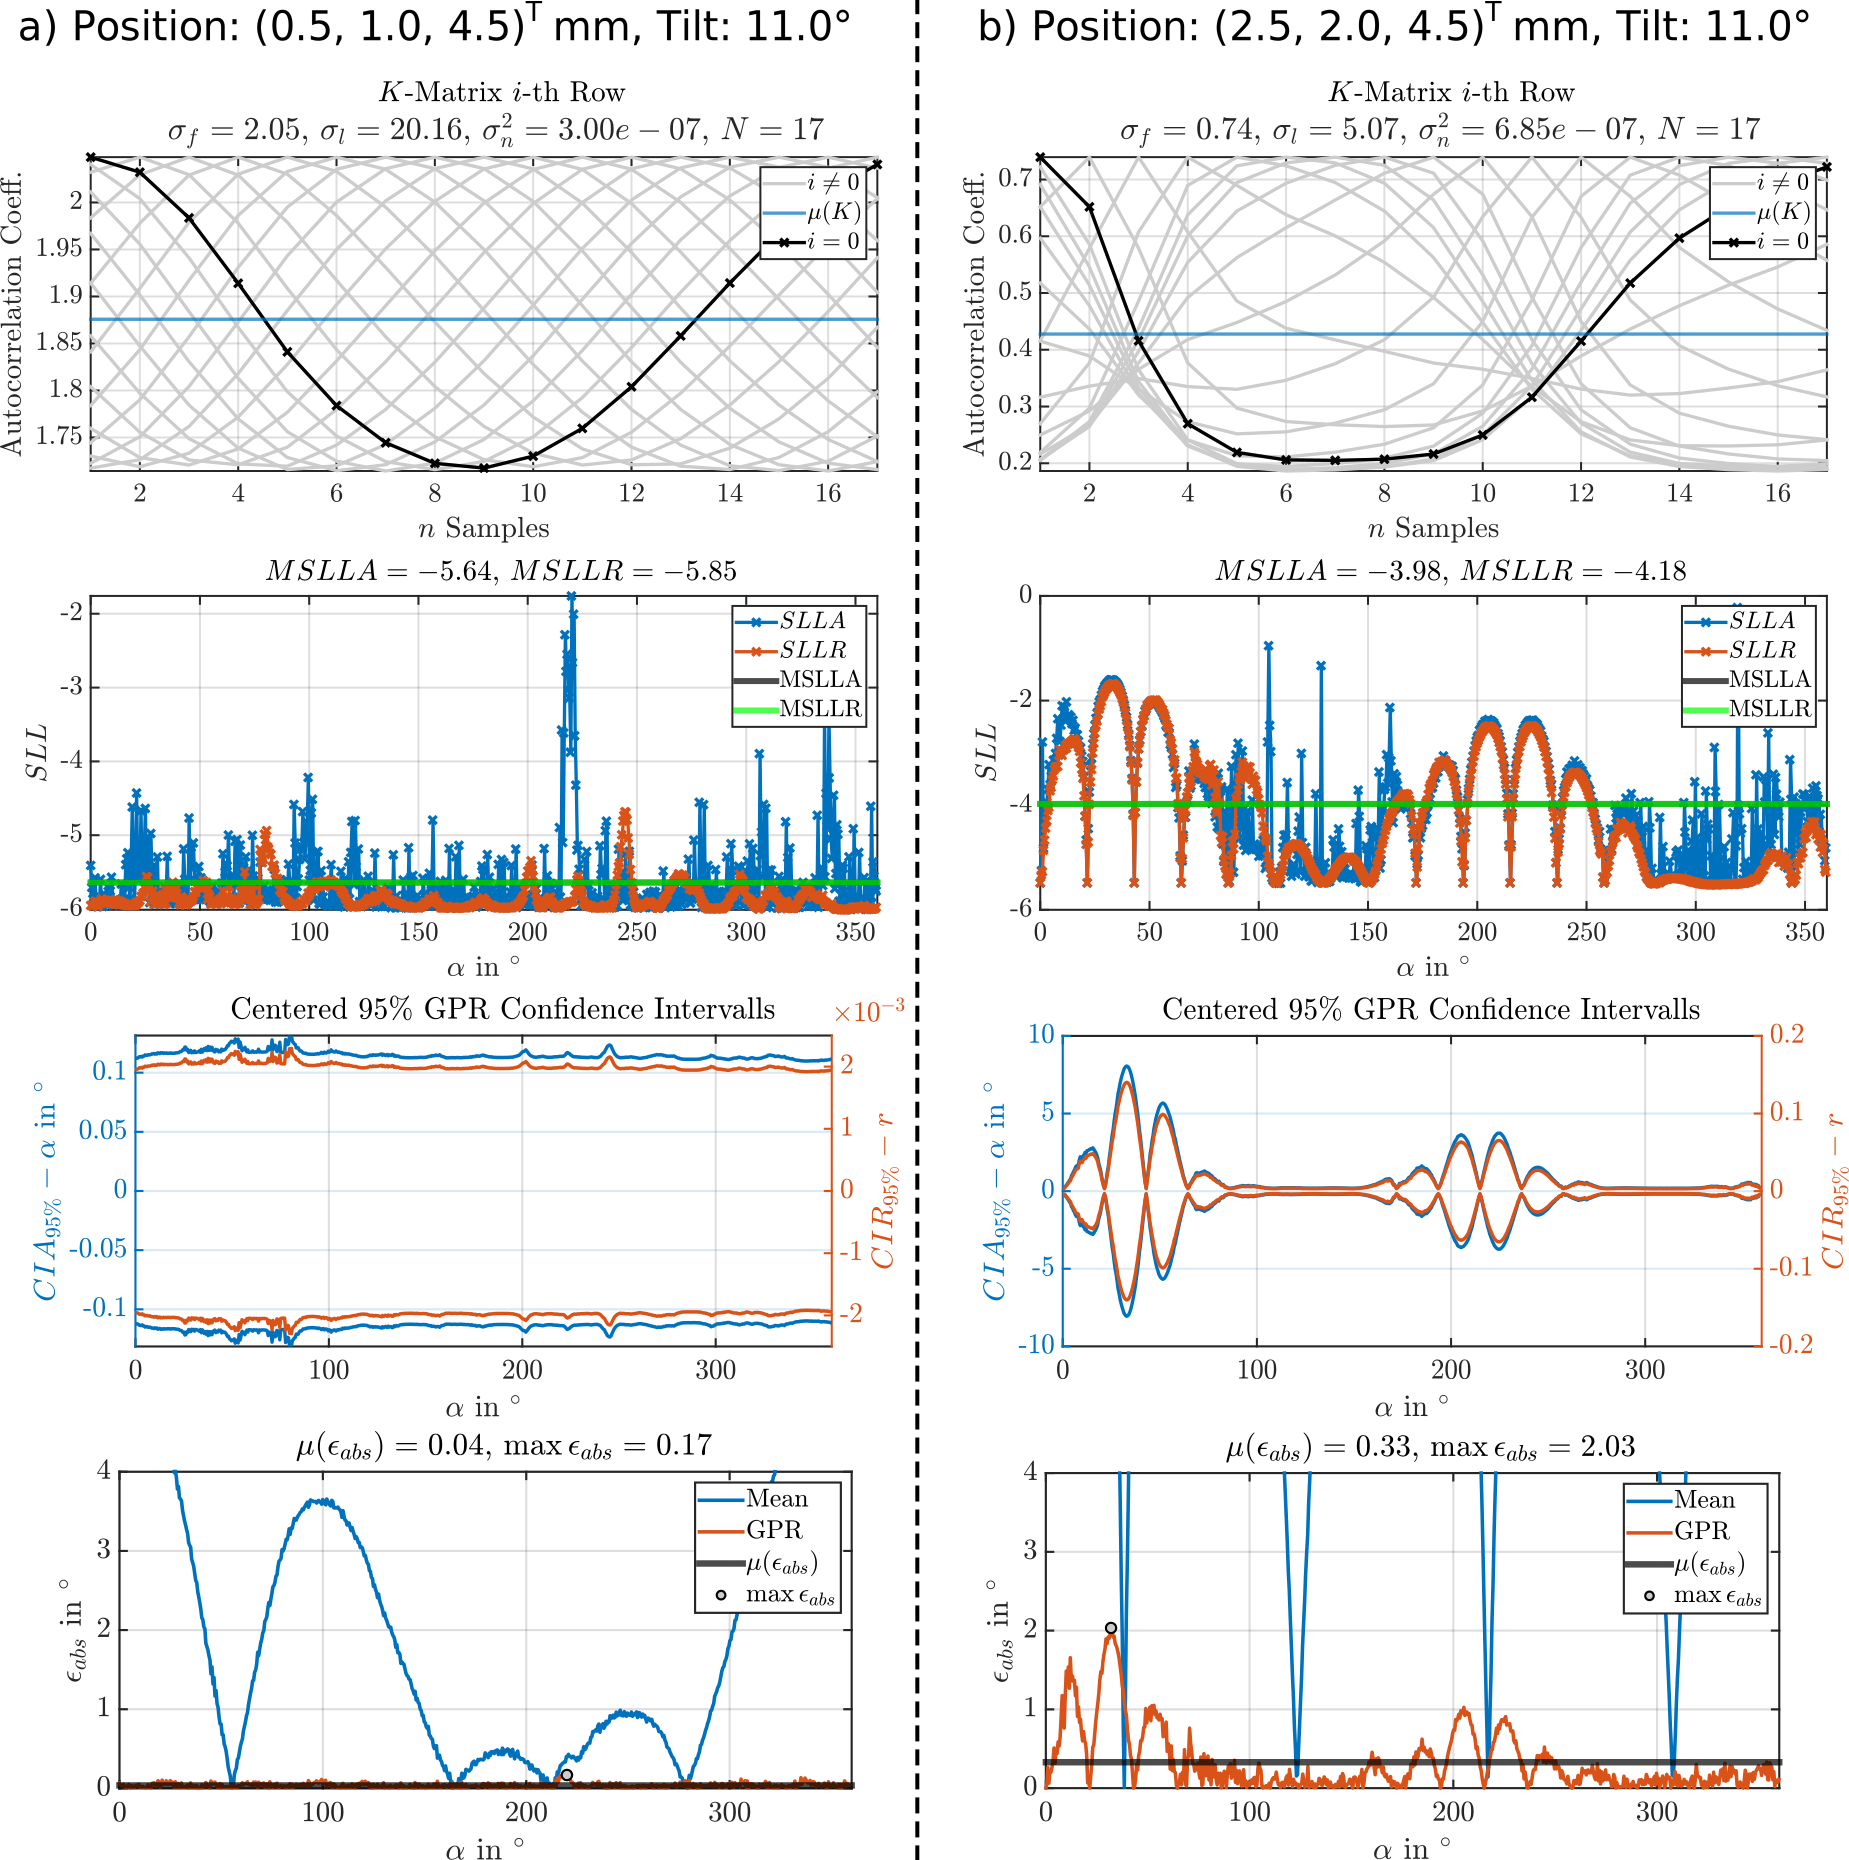
\includegraphics[width=\linewidth]{appendix/images/8-Ergebnisse-Experimente/Kombinierte-Fehllagen-GPR}
	\caption[Kombinierte Fehllagen Modell]{Kombinierte Fehllagen Modell}
	\label{fig:kombinierte-fehllagen-gpr}
\end{figure}



\begin{figure}[tbph]
	\centering
	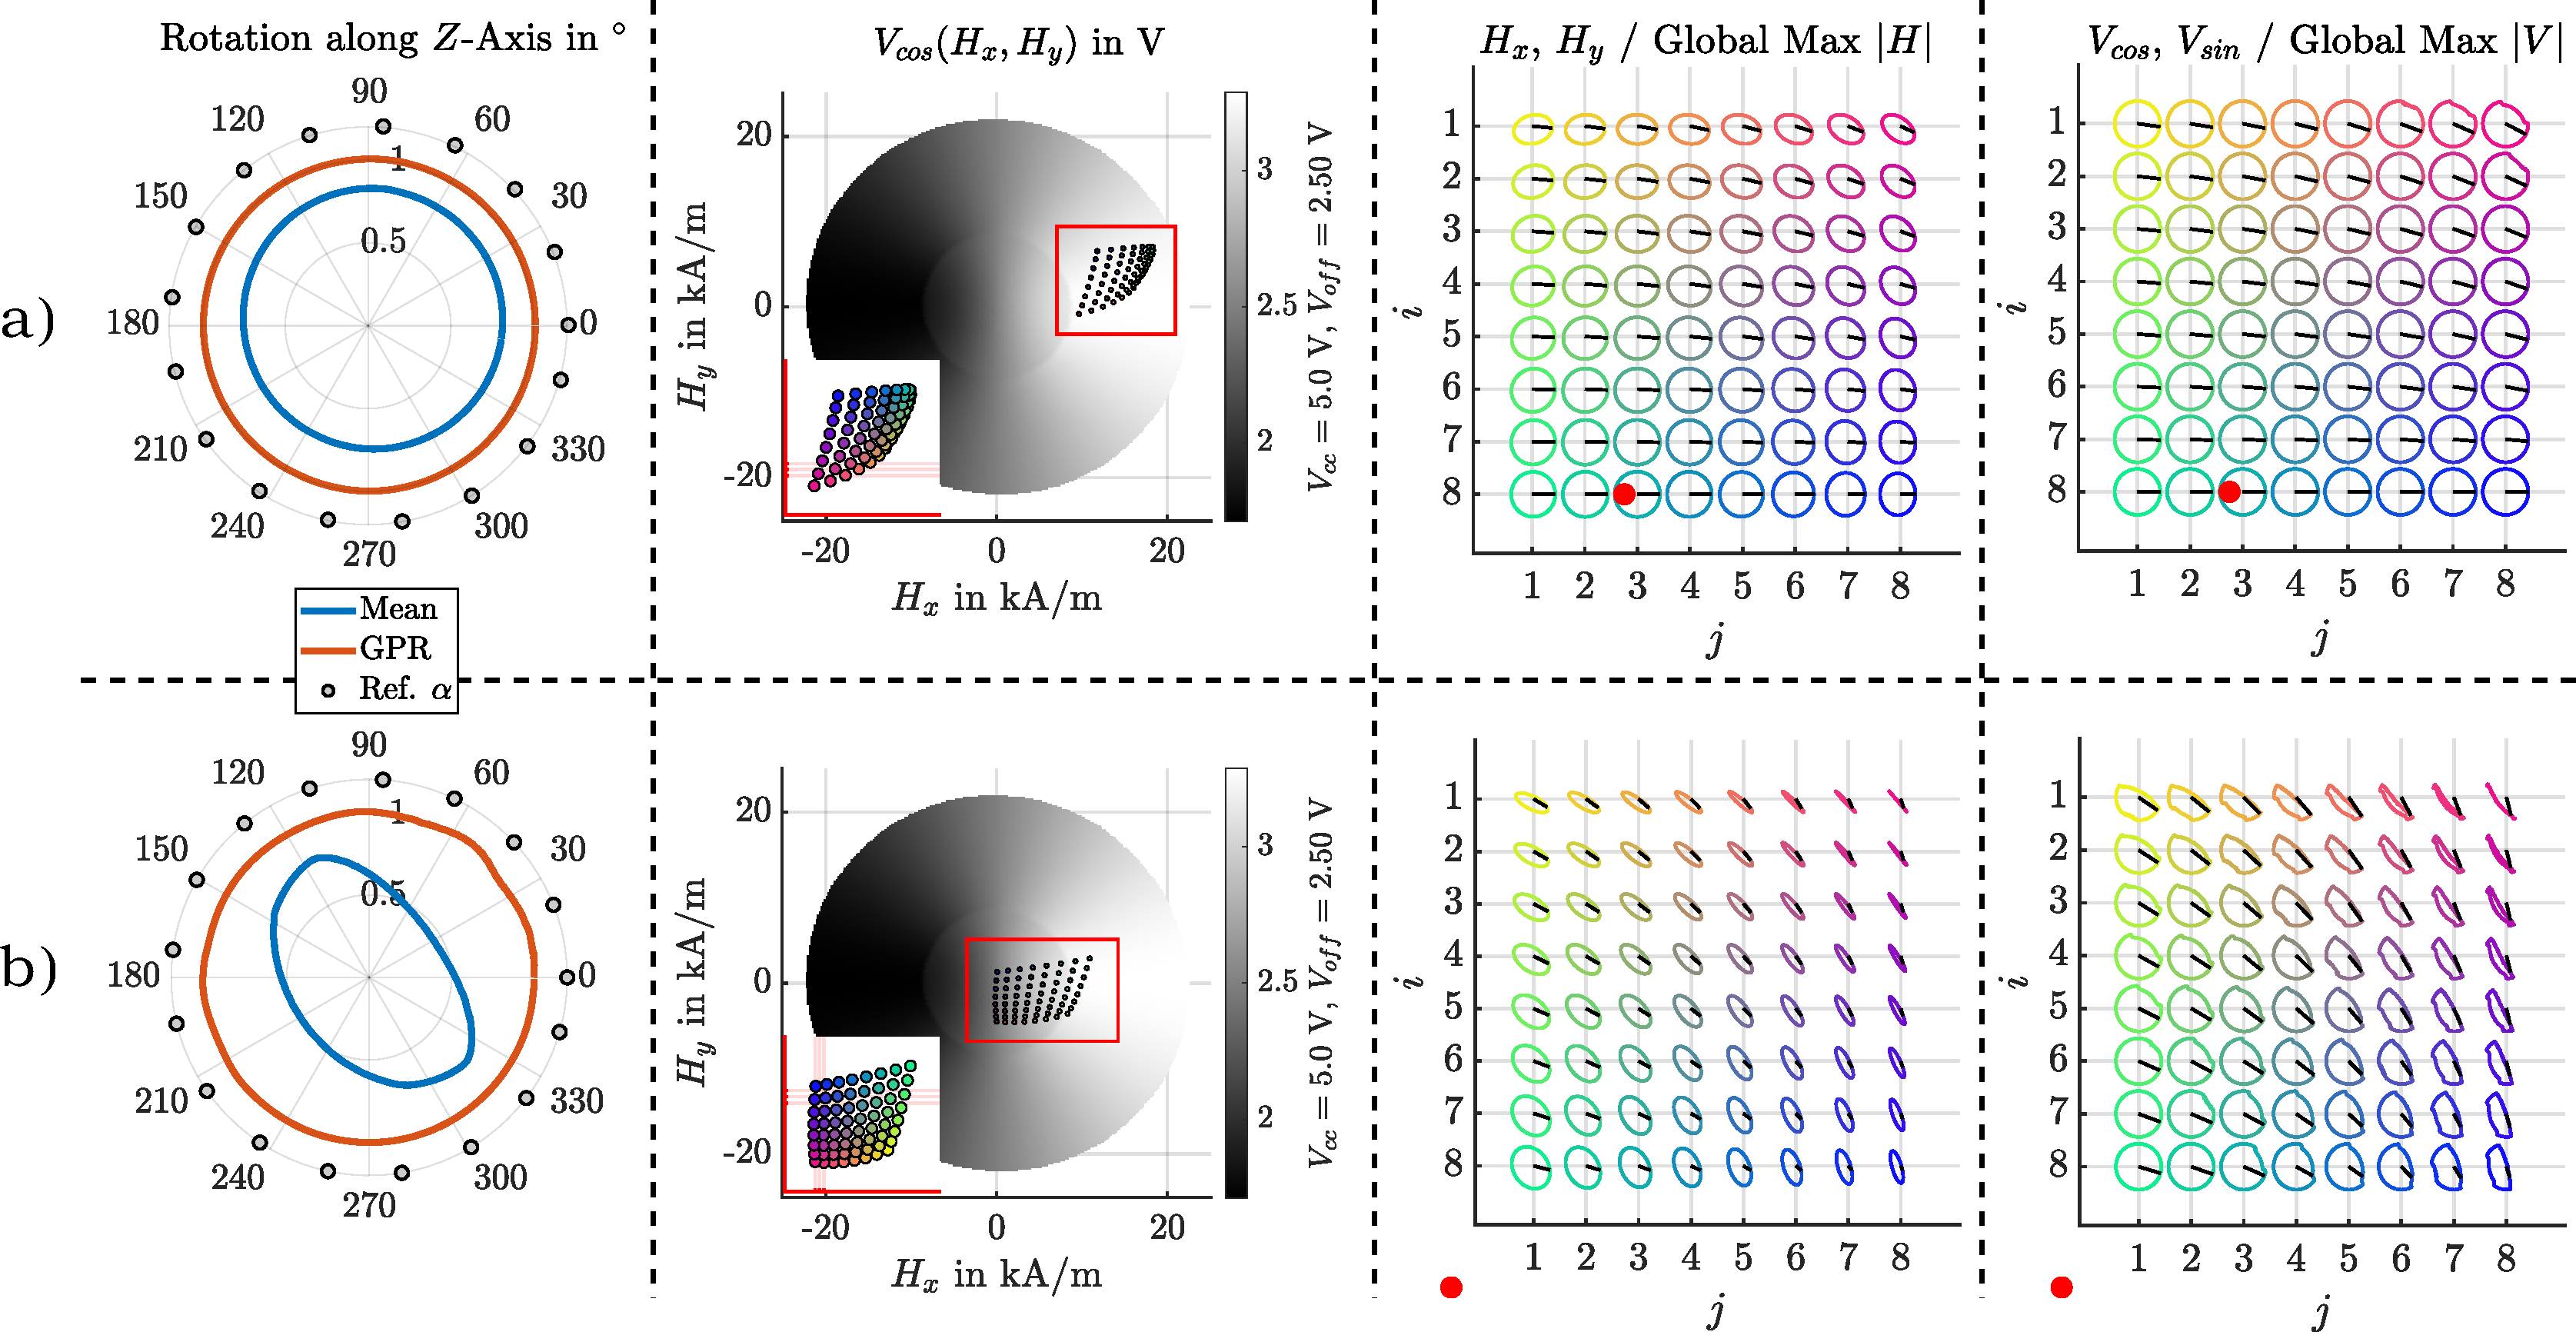
\includegraphics[width=\linewidth]{appendix/images/8-Ergebnisse-Experimente/Kombinierte-Fehllagen-Sensor}
	\caption[Kombinierte Fehlagen Sensor]{Kombinierte Fehlagen Sensor beide 11 tilt a) (0,0,4.5) b) (2.5,2,4.5) Verzerrung}
	\label{fig:kombinierte-fehllagen-sensor}
\end{figure}


